\documentclass[twoside]{book}

% Packages required by doxygen
\usepackage{fixltx2e}
\usepackage{calc}
\usepackage{doxygen}
\usepackage[export]{adjustbox} % also loads graphicx
\usepackage{graphicx}
\usepackage[utf8]{inputenc}
\usepackage{makeidx}
\usepackage{multicol}
\usepackage{multirow}
\PassOptionsToPackage{warn}{textcomp}
\usepackage{textcomp}
\usepackage[nointegrals]{wasysym}
\usepackage[table]{xcolor}

% Font selection
\usepackage[T1]{fontenc}
\usepackage[scaled=.90]{helvet}
\usepackage{courier}
\usepackage{amssymb}
\usepackage{sectsty}
\renewcommand{\familydefault}{\sfdefault}
\allsectionsfont{%
  \fontseries{bc}\selectfont%
  \color{darkgray}%
}
\renewcommand{\DoxyLabelFont}{%
  \fontseries{bc}\selectfont%
  \color{darkgray}%
}
\newcommand{\+}{\discretionary{\mbox{\scriptsize$\hookleftarrow$}}{}{}}

% Page & text layout
\usepackage{geometry}
\geometry{%
  a4paper,%
  top=2.5cm,%
  bottom=2.5cm,%
  left=2.5cm,%
  right=2.5cm%
}
\tolerance=750
\hfuzz=15pt
\hbadness=750
\setlength{\emergencystretch}{15pt}
\setlength{\parindent}{0cm}
\setlength{\parskip}{3ex plus 2ex minus 2ex}
\makeatletter
\renewcommand{\paragraph}{%
  \@startsection{paragraph}{4}{0ex}{-1.0ex}{1.0ex}{%
    \normalfont\normalsize\bfseries\SS@parafont%
  }%
}
\renewcommand{\subparagraph}{%
  \@startsection{subparagraph}{5}{0ex}{-1.0ex}{1.0ex}{%
    \normalfont\normalsize\bfseries\SS@subparafont%
  }%
}
\makeatother

% Headers & footers
\usepackage{fancyhdr}
\pagestyle{fancyplain}
\fancyhead[LE]{\fancyplain{}{\bfseries\thepage}}
\fancyhead[CE]{\fancyplain{}{}}
\fancyhead[RE]{\fancyplain{}{\bfseries\leftmark}}
\fancyhead[LO]{\fancyplain{}{\bfseries\rightmark}}
\fancyhead[CO]{\fancyplain{}{}}
\fancyhead[RO]{\fancyplain{}{\bfseries\thepage}}
\fancyfoot[LE]{\fancyplain{}{}}
\fancyfoot[CE]{\fancyplain{}{}}
\fancyfoot[RE]{\fancyplain{}{\bfseries\scriptsize Generated by Doxygen }}
\fancyfoot[LO]{\fancyplain{}{\bfseries\scriptsize Generated by Doxygen }}
\fancyfoot[CO]{\fancyplain{}{}}
\fancyfoot[RO]{\fancyplain{}{}}
\renewcommand{\footrulewidth}{0.4pt}
\renewcommand{\chaptermark}[1]{%
  \markboth{#1}{}%
}
\renewcommand{\sectionmark}[1]{%
  \markright{\thesection\ #1}%
}

% Indices & bibliography
\usepackage{natbib}
\usepackage[titles]{tocloft}
\setcounter{tocdepth}{3}
\setcounter{secnumdepth}{5}
\makeindex

% Hyperlinks (required, but should be loaded last)
\usepackage{ifpdf}
\ifpdf
  \usepackage[pdftex,pagebackref=true]{hyperref}
\else
  \usepackage[ps2pdf,pagebackref=true]{hyperref}
\fi
\hypersetup{%
  colorlinks=true,%
  linkcolor=blue,%
  citecolor=blue,%
  unicode%
}

% Custom commands
\newcommand{\clearemptydoublepage}{%
  \newpage{\pagestyle{empty}\cleardoublepage}%
}

\usepackage{caption}
\captionsetup{labelsep=space,justification=centering,font={bf},singlelinecheck=off,skip=4pt,position=top}

%===== C O N T E N T S =====

\begin{document}

% Titlepage & ToC
\hypersetup{pageanchor=false,
             bookmarksnumbered=true,
             pdfencoding=unicode
            }
\pagenumbering{roman}
\begin{titlepage}
\vspace*{7cm}
\begin{center}%
{\Large My Project }\\
\vspace*{1cm}
{\large Generated by Doxygen 1.8.11}\\
\end{center}
\end{titlepage}
\clearemptydoublepage
\tableofcontents
\clearemptydoublepage
\pagenumbering{arabic}
\hypersetup{pageanchor=true}

%--- Begin generated contents ---
\chapter{Hierarchical Index}
\section{Class Hierarchy}
This inheritance list is sorted roughly, but not completely, alphabetically\+:\begin{DoxyCompactList}
\item \contentsline{section}{Client}{\pageref{class_client}}{}
\item J\+Frame\begin{DoxyCompactList}
\item \contentsline{section}{Inf\+Sw}{\pageref{class_inf_sw}}{}
\end{DoxyCompactList}
\end{DoxyCompactList}

\chapter{Class Index}
\section{Class List}
Here are the classes, structs, unions and interfaces with brief descriptions\+:\begin{DoxyCompactList}
\item\contentsline{section}{\hyperlink{class_client}{Client} }{\pageref{class_client}}{}
\item\contentsline{section}{\hyperlink{class_inf_sw}{Inf\+Sw} }{\pageref{class_inf_sw}}{}
\end{DoxyCompactList}

\chapter{Class Documentation}
\hypertarget{class_base}{}\section{Base Class Reference}
\label{class_base}\index{Base@{Base}}
Inheritance diagram for Base\+:\begin{figure}[H]
\begin{center}
\leavevmode
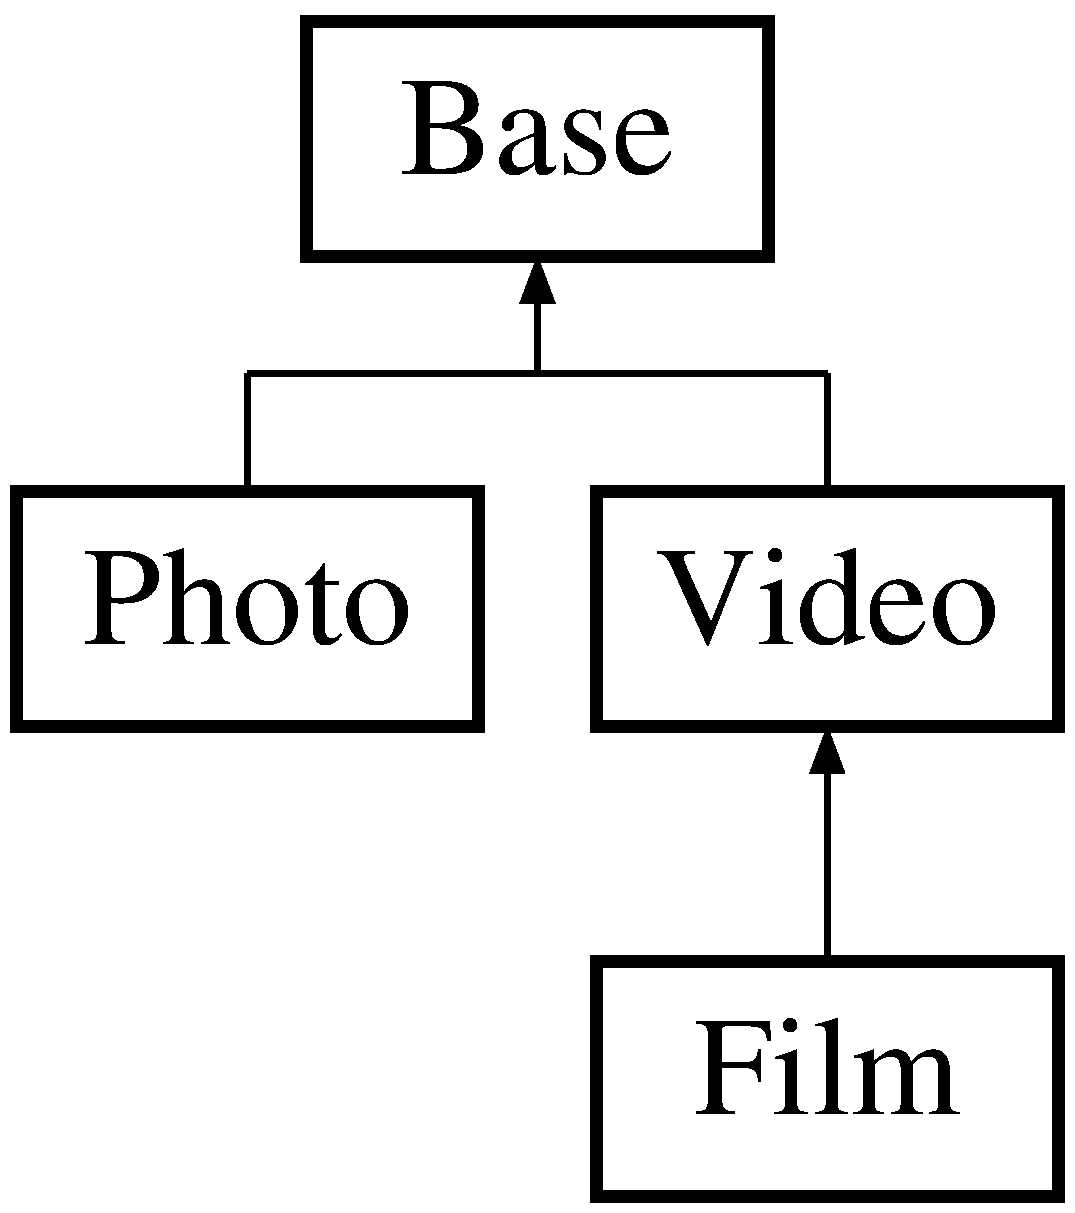
\includegraphics[height=3.000000cm]{class_base}
\end{center}
\end{figure}
\subsection*{Public Member Functions}
\begin{DoxyCompactItemize}
\item 
{\bfseries Base} (string obj, string pat)\hypertarget{class_base_a640c1141376d73d370b9ec15b254a515}{}\label{class_base_a640c1141376d73d370b9ec15b254a515}

\item 
virtual string {\bfseries get\+Object\+Name} () const \hypertarget{class_base_a518aecec79e084c1f49837c3cf1d0bad}{}\label{class_base_a518aecec79e084c1f49837c3cf1d0bad}

\item 
virtual string {\bfseries get\+Path\+Name} () const \hypertarget{class_base_a60d5c870af8cc2319ecb87abe520a23c}{}\label{class_base_a60d5c870af8cc2319ecb87abe520a23c}

\item 
virtual void {\bfseries set\+Object\+Name} (string obj)\hypertarget{class_base_a9f12058257f1d74f7c80854a239416b3}{}\label{class_base_a9f12058257f1d74f7c80854a239416b3}

\item 
virtual void {\bfseries set\+Path\+Name} (string pat)\hypertarget{class_base_af721d8940f7eb3cb0c72ba1155ce62c0}{}\label{class_base_af721d8940f7eb3cb0c72ba1155ce62c0}

\item 
virtual void {\bfseries print} (ostream \&os)\hypertarget{class_base_a8e0c44b66d66561fb1e10f5cc51459f2}{}\label{class_base_a8e0c44b66d66561fb1e10f5cc51459f2}

\item 
virtual void {\bfseries play} ()=0\hypertarget{class_base_a0a530a1710ef999953402c59e5df2861}{}\label{class_base_a0a530a1710ef999953402c59e5df2861}

\end{DoxyCompactItemize}
\subsection*{Protected Attributes}
\begin{DoxyCompactItemize}
\item 
string {\bfseries object\+Name}\hypertarget{class_base_a4493accaea84c12b7d658685cab8e4b4}{}\label{class_base_a4493accaea84c12b7d658685cab8e4b4}

\item 
string {\bfseries path\+Name}\hypertarget{class_base_ae04e87f86b2b19b5feaf62fc2957b0c1}{}\label{class_base_ae04e87f86b2b19b5feaf62fc2957b0c1}

\end{DoxyCompactItemize}


The documentation for this class was generated from the following files\+:\begin{DoxyCompactItemize}
\item 
C\+:/\+Users/\+Will/\+Desktop/\+Ung\+William/cpp/Base.\+h\item 
C\+:/\+Users/\+Will/\+Desktop/\+Ung\+William/cpp/Base.\+cpp\end{DoxyCompactItemize}

\hypertarget{class_t_c_p_server_1_1_callback}{}\section{T\+C\+P\+Server\+:\+:Callback Class Reference}
\label{class_t_c_p_server_1_1_callback}\index{T\+C\+P\+Server\+::\+Callback@{T\+C\+P\+Server\+::\+Callback}}
Inheritance diagram for T\+C\+P\+Server\+:\+:Callback\+:\begin{figure}[H]
\begin{center}
\leavevmode
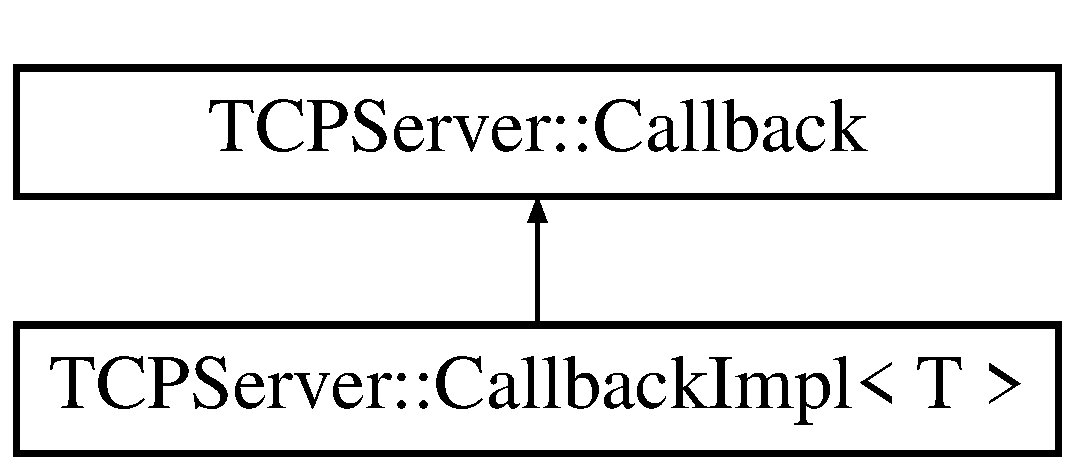
\includegraphics[height=2.000000cm]{class_t_c_p_server_1_1_callback}
\end{center}
\end{figure}
\subsection*{Public Member Functions}
\begin{DoxyCompactItemize}
\item 
virtual bool {\bfseries call\+Func} (\hyperlink{class_t_c_p_server_1_1_cnx}{Cnx} \&cnx, const std\+::string \&request, std\+::string \&response)=0\hypertarget{class_t_c_p_server_1_1_callback_a0d26469a5cfb3f5f0b3529cacb5d1615}{}\label{class_t_c_p_server_1_1_callback_a0d26469a5cfb3f5f0b3529cacb5d1615}

\end{DoxyCompactItemize}


The documentation for this class was generated from the following file\+:\begin{DoxyCompactItemize}
\item 
C\+:/\+Users/\+Will/\+Desktop/\+Ung\+William/cpp/T\+C\+P\+Server.\+h\end{DoxyCompactItemize}

\hypertarget{class_t_c_p_server_1_1_callback_impl}{}\section{T\+C\+P\+Server\+:\+:Callback\+Impl$<$ T $>$ Class Template Reference}
\label{class_t_c_p_server_1_1_callback_impl}\index{T\+C\+P\+Server\+::\+Callback\+Impl$<$ T $>$@{T\+C\+P\+Server\+::\+Callback\+Impl$<$ T $>$}}
Inheritance diagram for T\+C\+P\+Server\+:\+:Callback\+Impl$<$ T $>$\+:\begin{figure}[H]
\begin{center}
\leavevmode
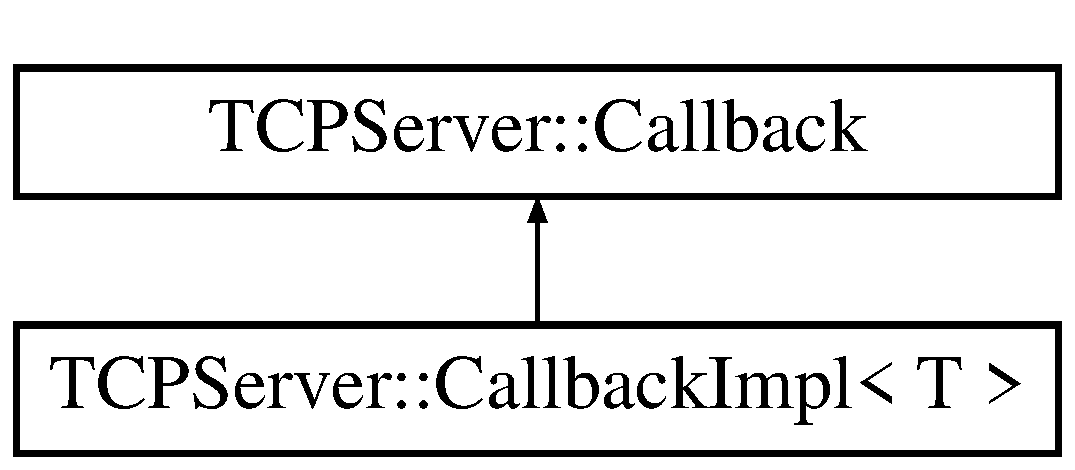
\includegraphics[height=2.000000cm]{class_t_c_p_server_1_1_callback_impl}
\end{center}
\end{figure}
\subsection*{Public Member Functions}
\begin{DoxyCompactItemize}
\item 
{\bfseries Callback\+Impl} (T $\ast$obj, Func func)\hypertarget{class_t_c_p_server_1_1_callback_impl_a39abe4ac0e2782d2ec0504a01fcdeb1e}{}\label{class_t_c_p_server_1_1_callback_impl_a39abe4ac0e2782d2ec0504a01fcdeb1e}

\item 
virtual bool {\bfseries call\+Func} (\hyperlink{class_t_c_p_server_1_1_cnx}{Cnx} \&cnx, const std\+::string \&request, std\+::string \&response)\hypertarget{class_t_c_p_server_1_1_callback_impl_a7370ad2f2dc50df8f623480f1991381b}{}\label{class_t_c_p_server_1_1_callback_impl_a7370ad2f2dc50df8f623480f1991381b}

\end{DoxyCompactItemize}


The documentation for this class was generated from the following file\+:\begin{DoxyCompactItemize}
\item 
C\+:/\+Users/\+Will/\+Desktop/\+Ung\+William/cpp/T\+C\+P\+Server.\+h\end{DoxyCompactItemize}

\hypertarget{class_t_c_p_server_1_1_cnx}{}\section{T\+C\+P\+Server\+:\+:Cnx Class Reference}
\label{class_t_c_p_server_1_1_cnx}\index{T\+C\+P\+Server\+::\+Cnx@{T\+C\+P\+Server\+::\+Cnx}}


represents a connection with a given client.  




{\ttfamily \#include $<$T\+C\+P\+Server.\+h$>$}

Inheritance diagram for T\+C\+P\+Server\+:\+:Cnx\+:\begin{figure}[H]
\begin{center}
\leavevmode
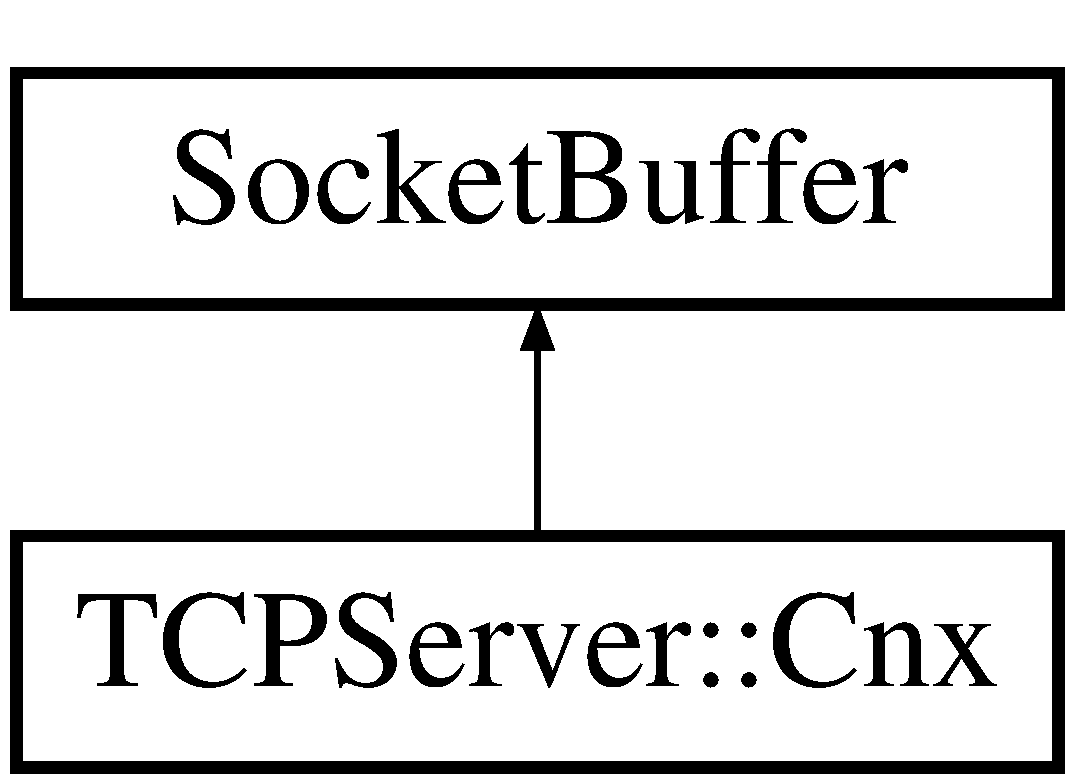
\includegraphics[height=2.000000cm]{class_t_c_p_server_1_1_cnx}
\end{center}
\end{figure}
\subsection*{Public Member Functions}
\begin{DoxyCompactItemize}
\item 
\hyperlink{class_t_c_p_server}{T\+C\+P\+Server} $\ast$ {\bfseries server} ()\hypertarget{class_t_c_p_server_1_1_cnx_affe5198f5dca75da9f651e286a289b47}{}\label{class_t_c_p_server_1_1_cnx_affe5198f5dca75da9f651e286a289b47}

\item 
pthread\+\_\+t {\bfseries thread} ()\hypertarget{class_t_c_p_server_1_1_cnx_a3dd1fff38f6463d62ef5f3cae4fad340}{}\label{class_t_c_p_server_1_1_cnx_a3dd1fff38f6463d62ef5f3cae4fad340}

\end{DoxyCompactItemize}
\subsection*{Friends}
\begin{DoxyCompactItemize}
\item 
class {\bfseries T\+C\+P\+Server}\hypertarget{class_t_c_p_server_1_1_cnx_ae4cfdb1814d91a8d28dadb49adda68f0}{}\label{class_t_c_p_server_1_1_cnx_ae4cfdb1814d91a8d28dadb49adda68f0}

\end{DoxyCompactItemize}
\subsection*{Additional Inherited Members}


\subsection{Detailed Description}
represents a connection with a given client. 

The documentation for this class was generated from the following files\+:\begin{DoxyCompactItemize}
\item 
C\+:/\+Users/\+Will/\+Desktop/\+Ung\+William/cpp/T\+C\+P\+Server.\+h\item 
C\+:/\+Users/\+Will/\+Desktop/\+Ung\+William/cpp/T\+C\+P\+Server.\+cpp\end{DoxyCompactItemize}

\hypertarget{class_film}{}\section{Film Class Reference}
\label{class_film}\index{Film@{Film}}
Inheritance diagram for Film\+:\begin{figure}[H]
\begin{center}
\leavevmode
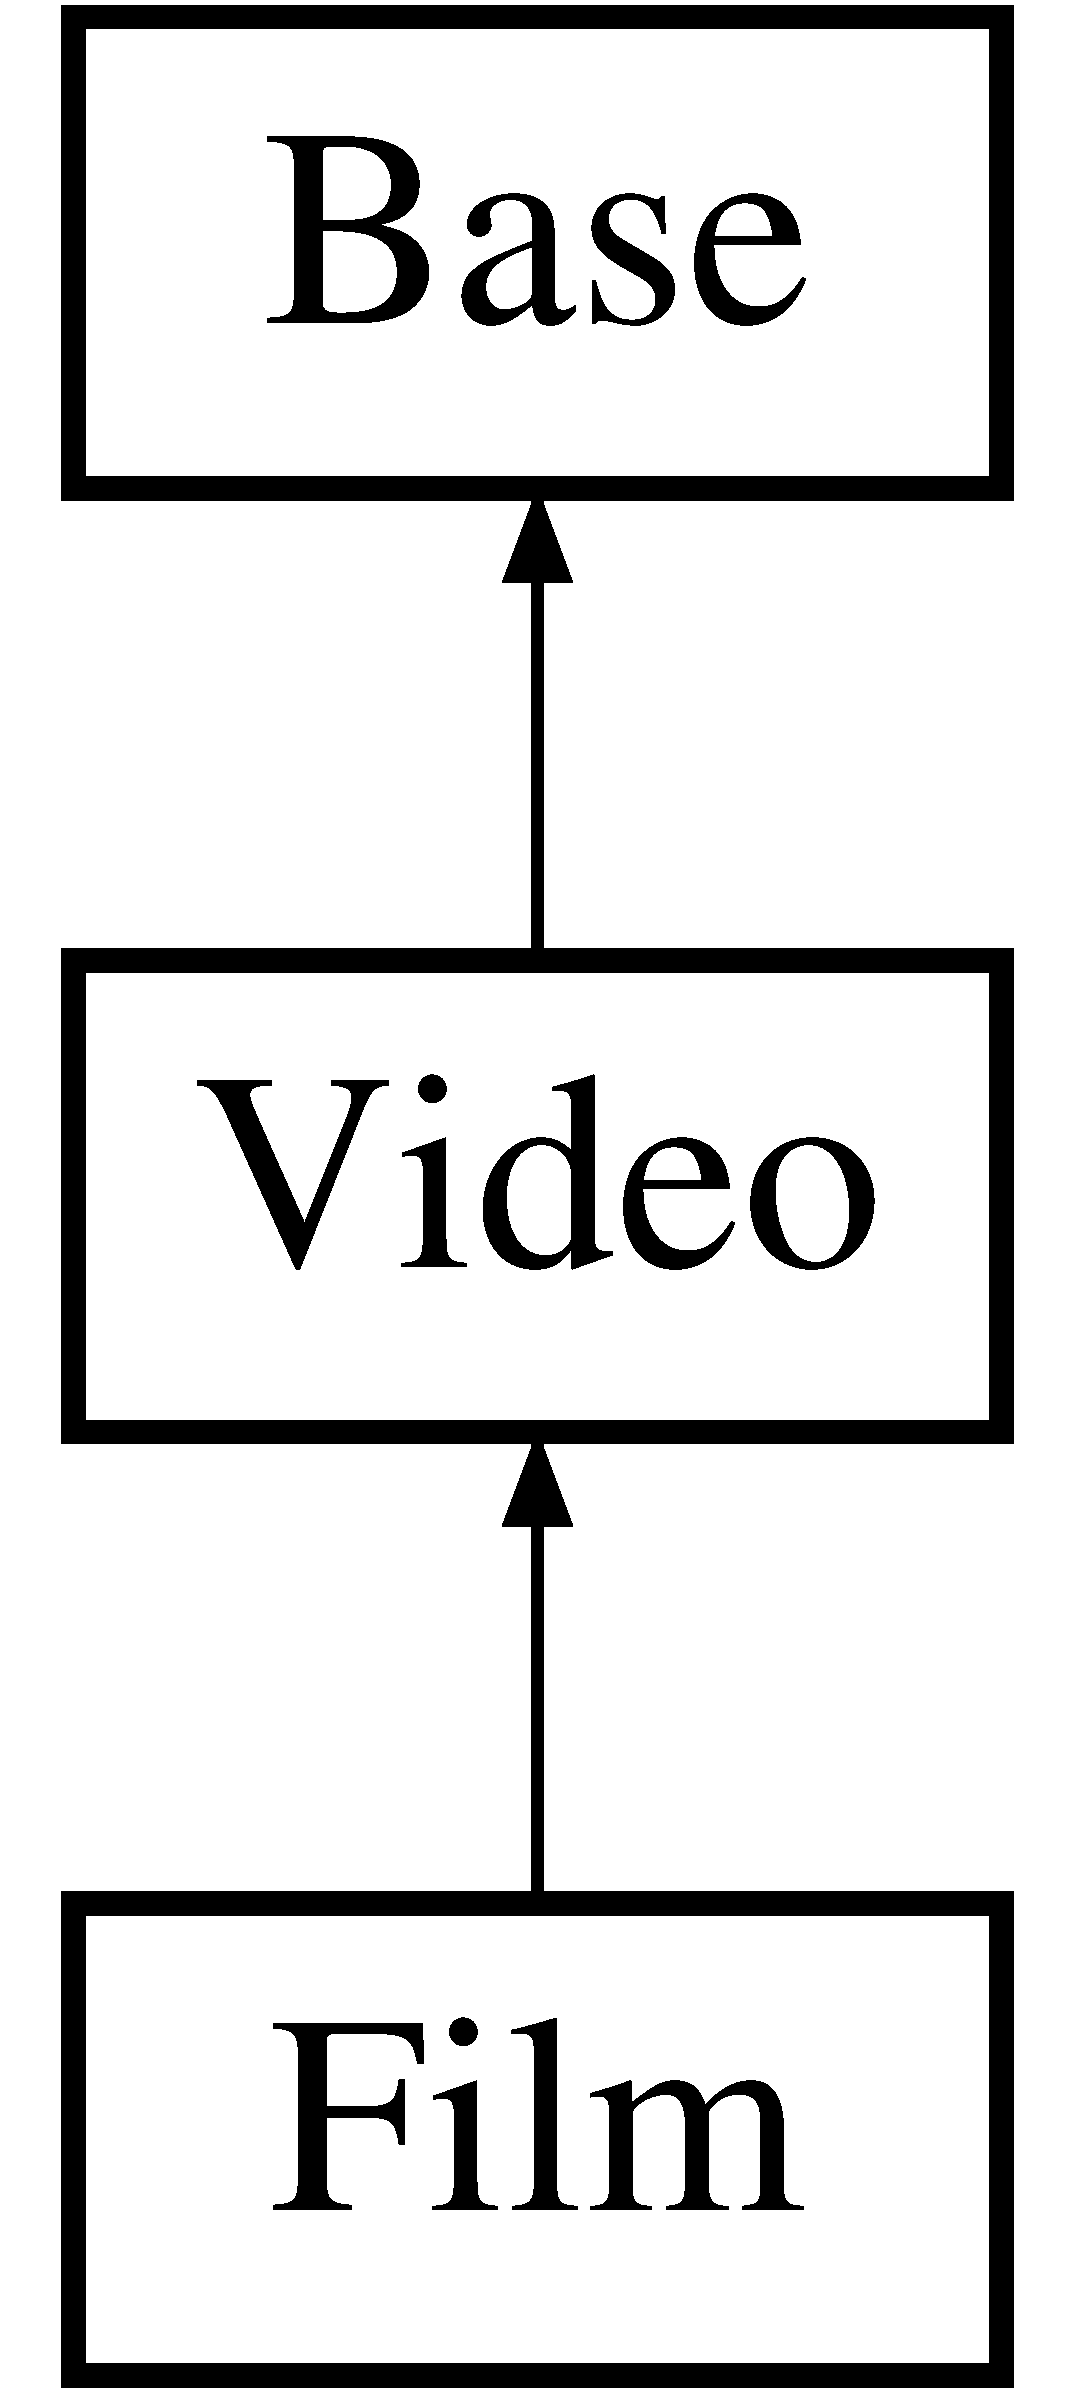
\includegraphics[height=3.000000cm]{class_film}
\end{center}
\end{figure}
\subsection*{Public Member Functions}
\begin{DoxyCompactItemize}
\item 
{\bfseries Film} (string \+\_\+obj, string \+\_\+pat, int \+\_\+duree, int $\ast$tab\+\_\+, int taille)\hypertarget{class_film_a9894b9e20dc8f5c5252743f53fe09bcb}{}\label{class_film_a9894b9e20dc8f5c5252743f53fe09bcb}

\item 
{\bfseries Film} (const \hyperlink{class_film}{Film} \&from)\hypertarget{class_film_a68f781851622ec80878c9a6e7ccb925e}{}\label{class_film_a68f781851622ec80878c9a6e7ccb925e}

\item 
virtual int $\ast$ {\bfseries get\+Tab} () const \hypertarget{class_film_ae05005bb993102212a5d1a0e5e582a2a}{}\label{class_film_ae05005bb993102212a5d1a0e5e582a2a}

\item 
virtual int {\bfseries get\+Nb\+Chap} () const \hypertarget{class_film_a750d6b5424e36ce2e28b2014a99decfd}{}\label{class_film_a750d6b5424e36ce2e28b2014a99decfd}

\item 
virtual void {\bfseries set\+Chap} (int $\ast$tab\+\_\+, int size\+\_\+)\hypertarget{class_film_a82a135c994d7fb715fad0ca72f9b75ee}{}\label{class_film_a82a135c994d7fb715fad0ca72f9b75ee}

\item 
virtual void {\bfseries print} (ostream \&os)\hypertarget{class_film_a7f1d7c74e51b17842adcd580c5e139ca}{}\label{class_film_a7f1d7c74e51b17842adcd580c5e139ca}

\end{DoxyCompactItemize}
\subsection*{Additional Inherited Members}


The documentation for this class was generated from the following files\+:\begin{DoxyCompactItemize}
\item 
C\+:/\+Users/\+Will/\+Desktop/\+Ung\+William/cpp/Film.\+h\item 
C\+:/\+Users/\+Will/\+Desktop/\+Ung\+William/cpp/Film.\+cpp\end{DoxyCompactItemize}

\hypertarget{class_groupe}{}\section{Groupe Class Reference}
\label{class_groupe}\index{Groupe@{Groupe}}
Inheritance diagram for Groupe\+:\begin{figure}[H]
\begin{center}
\leavevmode
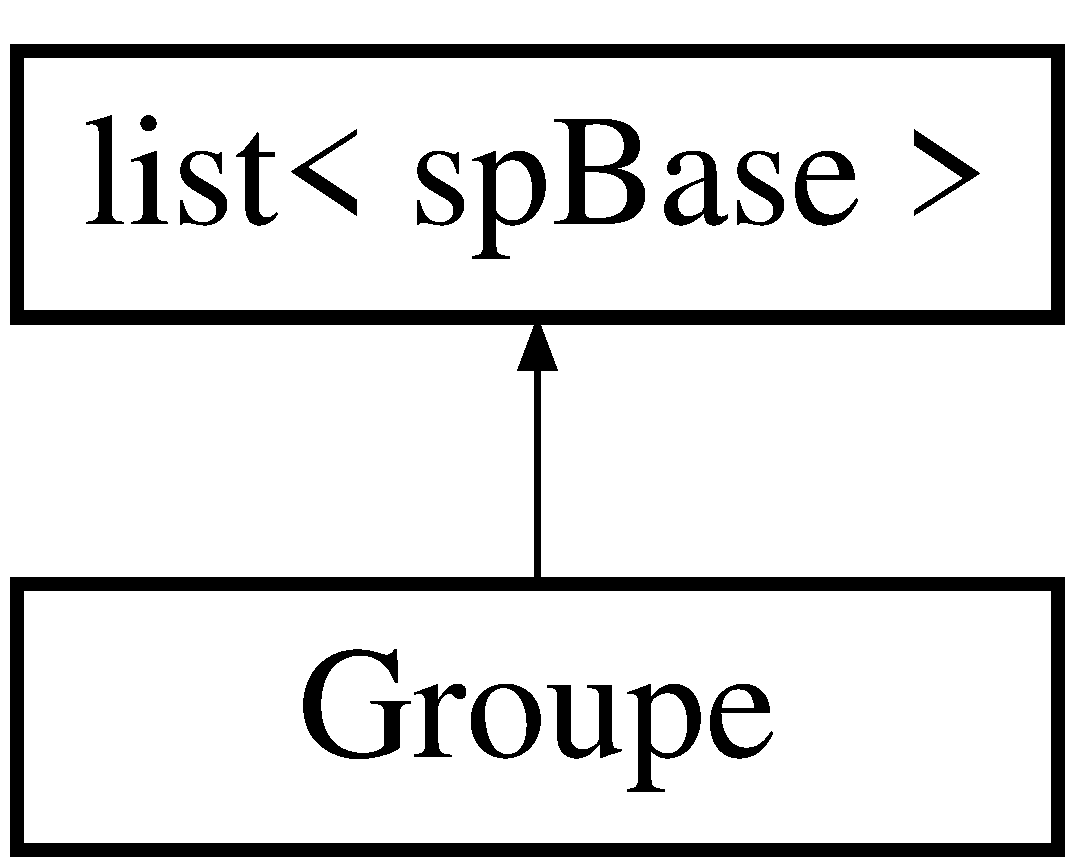
\includegraphics[height=2.000000cm]{class_groupe}
\end{center}
\end{figure}
\subsection*{Public Member Functions}
\begin{DoxyCompactItemize}
\item 
{\bfseries Groupe} (string \+\_\+name)\hypertarget{class_groupe_ad4cd49f43b43c2a0abfc7b283f37e9bc}{}\label{class_groupe_ad4cd49f43b43c2a0abfc7b283f37e9bc}

\item 
virtual string {\bfseries get\+Name} () const \hypertarget{class_groupe_a59bb4c47682eaee83c9e602e77a2fe68}{}\label{class_groupe_a59bb4c47682eaee83c9e602e77a2fe68}

\item 
virtual void {\bfseries print} (ostream \&os)\hypertarget{class_groupe_a9f0f019a28fbe9ba503bfbe184985d2a}{}\label{class_groupe_a9f0f019a28fbe9ba503bfbe184985d2a}

\item 
virtual void {\bfseries add\+Base} (sp\+Base b)\hypertarget{class_groupe_ab1f6b10655bc77873472c72a1b9d06b0}{}\label{class_groupe_ab1f6b10655bc77873472c72a1b9d06b0}

\item 
virtual void {\bfseries remove\+Base} (sp\+Base b)\hypertarget{class_groupe_a79bd65c60555e37ce18e6dc15fa56a60}{}\label{class_groupe_a79bd65c60555e37ce18e6dc15fa56a60}

\end{DoxyCompactItemize}
\subsection*{Protected Attributes}
\begin{DoxyCompactItemize}
\item 
string {\bfseries name}\hypertarget{class_groupe_a45d675668955ce1509a3bbce8fb7e82c}{}\label{class_groupe_a45d675668955ce1509a3bbce8fb7e82c}

\end{DoxyCompactItemize}


The documentation for this class was generated from the following files\+:\begin{DoxyCompactItemize}
\item 
C\+:/\+Users/\+Will/\+Desktop/\+Ung\+William/cpp/Groupe.\+h\item 
C\+:/\+Users/\+Will/\+Desktop/\+Ung\+William/cpp/Groupe.\+cpp\end{DoxyCompactItemize}

\hypertarget{struct_input_buffer}{}\section{Input\+Buffer Struct Reference}
\label{struct_input_buffer}\index{Input\+Buffer@{Input\+Buffer}}
\subsection*{Public Member Functions}
\begin{DoxyCompactItemize}
\item 
{\bfseries Input\+Buffer} (size\+\_\+t size)\hypertarget{struct_input_buffer_a9409ec8e4581caa99dcac1af963349b5}{}\label{struct_input_buffer_a9409ec8e4581caa99dcac1af963349b5}

\end{DoxyCompactItemize}
\subsection*{Public Attributes}
\begin{DoxyCompactItemize}
\item 
char $\ast$ {\bfseries buffer}\hypertarget{struct_input_buffer_aee7a717b6cf023deabe9910410e6cfb6}{}\label{struct_input_buffer_aee7a717b6cf023deabe9910410e6cfb6}

\item 
char $\ast$ {\bfseries begin}\hypertarget{struct_input_buffer_a2f05121c4fb8571845cc22d083c6da46}{}\label{struct_input_buffer_a2f05121c4fb8571845cc22d083c6da46}

\item 
char $\ast$ {\bfseries end}\hypertarget{struct_input_buffer_a52ba71c71b9b955b8369fc5217e3c4b6}{}\label{struct_input_buffer_a52ba71c71b9b955b8369fc5217e3c4b6}

\item 
ssize\+\_\+t {\bfseries remaining}\hypertarget{struct_input_buffer_a621d633184a77c449e7b07d705870ae2}{}\label{struct_input_buffer_a621d633184a77c449e7b07d705870ae2}

\end{DoxyCompactItemize}


The documentation for this struct was generated from the following file\+:\begin{DoxyCompactItemize}
\item 
C\+:/\+Users/\+Will/\+Desktop/\+Ung\+William/cpp/Socket.\+cpp\end{DoxyCompactItemize}

\hypertarget{class_t_c_p_server_1_1_lock}{}\section{T\+C\+P\+Server\+:\+:Lock Class Reference}
\label{class_t_c_p_server_1_1_lock}\index{T\+C\+P\+Server\+::\+Lock@{T\+C\+P\+Server\+::\+Lock}}


locks the server in read mode or in write mode. In order to avoid concurrency problems between threads, the callback method that processes requests should instantiate a \hyperlink{class_t_c_p_server_1_1_lock}{Lock} object in the stack. The \hyperlink{class_t_c_p_server_1_1_lock}{Lock} must be instantiated in write mode if the request changes data, or in read mode otherwise. A write lock blocks all other locks (hence, all other threads) until the callback method that issued the write lock returns.  




{\ttfamily \#include $<$T\+C\+P\+Server.\+h$>$}

\subsection*{Public Member Functions}
\begin{DoxyCompactItemize}
\item 
\hyperlink{class_t_c_p_server_1_1_lock_a4b1fa591dde407aacd93133828cfac81}{Lock} (\hyperlink{class_t_c_p_server_1_1_cnx}{Cnx} \&, bool write\+Mode=false)\hypertarget{class_t_c_p_server_1_1_lock_a4b1fa591dde407aacd93133828cfac81}{}\label{class_t_c_p_server_1_1_lock_a4b1fa591dde407aacd93133828cfac81}

\begin{DoxyCompactList}\small\item\em locks the connection in write mode if the second argument is true and in read mode otherwise. \end{DoxyCompactList}\end{DoxyCompactItemize}


\subsection{Detailed Description}
locks the server in read mode or in write mode. In order to avoid concurrency problems between threads, the callback method that processes requests should instantiate a \hyperlink{class_t_c_p_server_1_1_lock}{Lock} object in the stack. The \hyperlink{class_t_c_p_server_1_1_lock}{Lock} must be instantiated in write mode if the request changes data, or in read mode otherwise. A write lock blocks all other locks (hence, all other threads) until the callback method that issued the write lock returns. 

The documentation for this class was generated from the following files\+:\begin{DoxyCompactItemize}
\item 
C\+:/\+Users/\+Will/\+Desktop/\+Ung\+William/cpp/T\+C\+P\+Server.\+h\item 
C\+:/\+Users/\+Will/\+Desktop/\+Ung\+William/cpp/T\+C\+P\+Server.\+cpp\end{DoxyCompactItemize}

\hypertarget{class_photo}{}\section{Photo Class Reference}
\label{class_photo}\index{Photo@{Photo}}
Inheritance diagram for Photo\+:\begin{figure}[H]
\begin{center}
\leavevmode
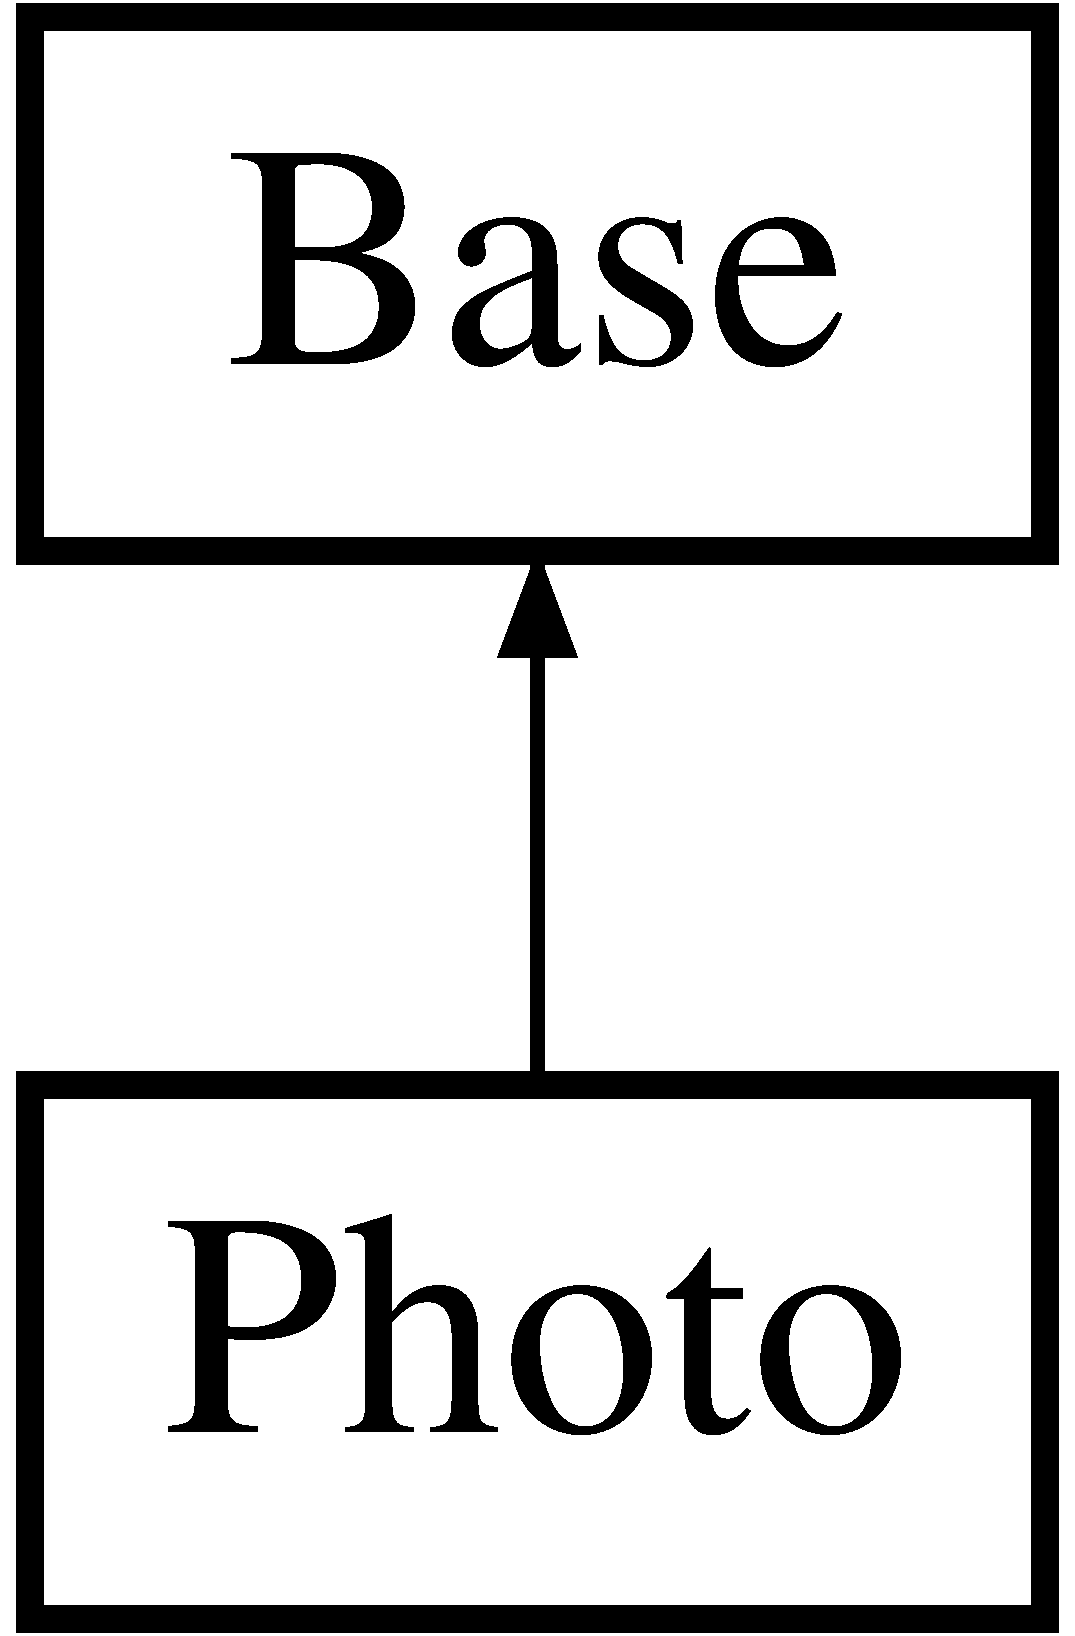
\includegraphics[height=2.000000cm]{class_photo}
\end{center}
\end{figure}
\subsection*{Public Member Functions}
\begin{DoxyCompactItemize}
\item 
{\bfseries Photo} (string obj, string pat, float \+\_\+wid=0, float \+\_\+hei=0)\hypertarget{class_photo_a1b8648212e291ecee50c9d43e8383cfc}{}\label{class_photo_a1b8648212e291ecee50c9d43e8383cfc}

\item 
float {\bfseries get\+Wid} () const \hypertarget{class_photo_ac98a0affa9a26d288cc69929ce8940b7}{}\label{class_photo_ac98a0affa9a26d288cc69929ce8940b7}

\item 
float {\bfseries get\+Hei} () const \hypertarget{class_photo_adaa07219604bb7330eb29e90a5f584ce}{}\label{class_photo_adaa07219604bb7330eb29e90a5f584ce}

\item 
void {\bfseries set\+Wid} (float wi)\hypertarget{class_photo_a022cfb5b882184ddc999bb82484f13be}{}\label{class_photo_a022cfb5b882184ddc999bb82484f13be}

\item 
void {\bfseries set\+Hei} (float he)\hypertarget{class_photo_a5084839d44991247d9127ad8404fba85}{}\label{class_photo_a5084839d44991247d9127ad8404fba85}

\item 
virtual void {\bfseries print} (ostream \&os) override\hypertarget{class_photo_ac0d0e8276f3f5cf020bdde5b115fd017}{}\label{class_photo_ac0d0e8276f3f5cf020bdde5b115fd017}

\item 
virtual void {\bfseries play} () override\hypertarget{class_photo_a38cc8ab7ab354411e2fb49642880b373}{}\label{class_photo_a38cc8ab7ab354411e2fb49642880b373}

\end{DoxyCompactItemize}
\subsection*{Protected Attributes}
\begin{DoxyCompactItemize}
\item 
float {\bfseries wid}\hypertarget{class_photo_a4f4048eed34821248f4c3be53cedd544}{}\label{class_photo_a4f4048eed34821248f4c3be53cedd544}

\item 
float {\bfseries hei}\hypertarget{class_photo_a999ec71ceb2c57ed25053c2cbcdc225e}{}\label{class_photo_a999ec71ceb2c57ed25053c2cbcdc225e}

\end{DoxyCompactItemize}


The documentation for this class was generated from the following file\+:\begin{DoxyCompactItemize}
\item 
C\+:/\+Users/\+Will/\+Desktop/\+Ung\+William/cpp/Photo.\+h\end{DoxyCompactItemize}

\hypertarget{class_server_socket}{}\section{Server\+Socket Class Reference}
\label{class_server_socket}\index{Server\+Socket@{Server\+Socket}}


T\+C\+P/\+IP \hyperlink{class_socket}{Socket} Server. This class encapsulates a T\+C\+P/\+IP socket server. A\+F\+\_\+\+I\+N\+ET connections following the I\+Pv4 Internet protocol are supported.  




{\ttfamily \#include $<$Socket.\+h$>$}

\subsection*{Public Member Functions}
\begin{DoxyCompactItemize}
\item 
\hyperlink{class_server_socket_a2b3098589541243241ca25495155186c}{Server\+Socket} ()\hypertarget{class_server_socket_a2b3098589541243241ca25495155186c}{}\label{class_server_socket_a2b3098589541243241ca25495155186c}

\begin{DoxyCompactList}\small\item\em Creates a new server socket. Creates a listening socket that waits for connection requests by T\+C\+P/\+IP clients. \end{DoxyCompactList}\item 
virtual \hyperlink{class_socket}{Socket} $\ast$ \hyperlink{class_server_socket_accc3d56d42aa50a5f3c920cf0b26959b}{accept} ()
\begin{DoxyCompactList}\small\item\em Accepts a new connection request and returns the corresponding socket. By default, this function blocks the caller until a connection is present. \end{DoxyCompactList}\item 
virtual int \hyperlink{class_server_socket_ad5281fe6c005bca007a9a758bd612481}{bind} (int port, int backlog=50)
\begin{DoxyCompactList}\small\item\em Assigns the socket to the local address. The socket must be bound before using it. \end{DoxyCompactList}\item 
virtual int \hyperlink{class_server_socket_a3eac6d5571bb092622d328dbda2de2cf}{close} ()\hypertarget{class_server_socket_a3eac6d5571bb092622d328dbda2de2cf}{}\label{class_server_socket_a3eac6d5571bb092622d328dbda2de2cf}

\begin{DoxyCompactList}\small\item\em Closes the socket. \end{DoxyCompactList}\item 
bool \hyperlink{class_server_socket_ad5b053b711f97cfe8b56f6febc15df65}{is\+Closed} () const \hypertarget{class_server_socket_ad5b053b711f97cfe8b56f6febc15df65}{}\label{class_server_socket_ad5b053b711f97cfe8b56f6febc15df65}

\begin{DoxyCompactList}\small\item\em Returns true if the socket has been closed. \end{DoxyCompactList}\item 
int \hyperlink{class_server_socket_a57b5b84a60906153d9755190cdfd0d39}{descriptor} ()\hypertarget{class_server_socket_a57b5b84a60906153d9755190cdfd0d39}{}\label{class_server_socket_a57b5b84a60906153d9755190cdfd0d39}

\begin{DoxyCompactList}\small\item\em Returns the Unix descriptor of the socket. \end{DoxyCompactList}\item 
int \hyperlink{class_server_socket_ab34154bc6114c638ae02f5e018121099}{set\+Receive\+Buffer\+Size} (int size)\hypertarget{class_server_socket_ab34154bc6114c638ae02f5e018121099}{}\label{class_server_socket_ab34154bc6114c638ae02f5e018121099}

\begin{DoxyCompactList}\small\item\em Sets the S\+O\+\_\+\+R\+C\+V\+B\+UF option to the specified value. \end{DoxyCompactList}\item 
int \hyperlink{class_server_socket_ae60d7cc31ad535e5d3cac42e38b8ec98}{set\+Reuse\+Address} (bool)\hypertarget{class_server_socket_ae60d7cc31ad535e5d3cac42e38b8ec98}{}\label{class_server_socket_ae60d7cc31ad535e5d3cac42e38b8ec98}

\begin{DoxyCompactList}\small\item\em Enables/disables the S\+O\+\_\+\+R\+E\+U\+S\+E\+A\+D\+DR socket option. \end{DoxyCompactList}\item 
int \hyperlink{class_server_socket_aedb9144c9c375fcb14ac47bcb9d2eb17}{set\+So\+Timeout} (int timeout)\hypertarget{class_server_socket_aedb9144c9c375fcb14ac47bcb9d2eb17}{}\label{class_server_socket_aedb9144c9c375fcb14ac47bcb9d2eb17}

\begin{DoxyCompactList}\small\item\em Enables/disables S\+O\+\_\+\+T\+I\+M\+E\+O\+UT with the specified timeout (in milliseconds). \end{DoxyCompactList}\item 
int \hyperlink{class_server_socket_a9e5e1ee852ba26156c757a0086b780fe}{set\+Tcp\+No\+Delay} (bool)\hypertarget{class_server_socket_a9e5e1ee852ba26156c757a0086b780fe}{}\label{class_server_socket_a9e5e1ee852ba26156c757a0086b780fe}

\begin{DoxyCompactList}\small\item\em Turns on/off T\+CP coalescence (useful in some cases to avoid delays). \end{DoxyCompactList}\end{DoxyCompactItemize}


\subsection{Detailed Description}
T\+C\+P/\+IP \hyperlink{class_socket}{Socket} Server. This class encapsulates a T\+C\+P/\+IP socket server. A\+F\+\_\+\+I\+N\+ET connections following the I\+Pv4 Internet protocol are supported. 

Class \hyperlink{class_socket}{Socket} should be used on the client side (\begin{DoxySeeAlso}{See also}
\hyperlink{class_socket}{Socket}).
\end{DoxySeeAlso}
T\+C\+P/\+IP sockets do not preserve record boundaries, \begin{DoxySeeAlso}{See also}
\hyperlink{class_socket_buffer}{Socket\+Buffer} for a solution. 
\end{DoxySeeAlso}


\subsection{Member Function Documentation}
\index{Server\+Socket@{Server\+Socket}!accept@{accept}}
\index{accept@{accept}!Server\+Socket@{Server\+Socket}}
\subsubsection[{\texorpdfstring{accept()}{accept()}}]{\setlength{\rightskip}{0pt plus 5cm}{\bf Socket} $\ast$ Server\+Socket\+::accept (
\begin{DoxyParamCaption}
{}
\end{DoxyParamCaption}
)\hspace{0.3cm}{\ttfamily [virtual]}}\hypertarget{class_server_socket_accc3d56d42aa50a5f3c920cf0b26959b}{}\label{class_server_socket_accc3d56d42aa50a5f3c920cf0b26959b}


Accepts a new connection request and returns the corresponding socket. By default, this function blocks the caller until a connection is present. 

\begin{DoxyReturn}{Returns}
the new \hyperlink{class_socket}{Socket} or nullptr on error. 
\end{DoxyReturn}
\index{Server\+Socket@{Server\+Socket}!bind@{bind}}
\index{bind@{bind}!Server\+Socket@{Server\+Socket}}
\subsubsection[{\texorpdfstring{bind(int port, int backlog=50)}{bind(int port, int backlog=50)}}]{\setlength{\rightskip}{0pt plus 5cm}int Server\+Socket\+::bind (
\begin{DoxyParamCaption}
\item[{int}]{port, }
\item[{int}]{backlog = {\ttfamily 50}}
\end{DoxyParamCaption}
)\hspace{0.3cm}{\ttfamily [virtual]}}\hypertarget{class_server_socket_ad5281fe6c005bca007a9a758bd612481}{}\label{class_server_socket_ad5281fe6c005bca007a9a758bd612481}


Assigns the socket to the local address. The socket must be bound before using it. 

\begin{DoxyReturn}{Returns}
0 on success or a negative value on error which is one of \hyperlink{class_socket_a9f68308228badcdd299cd83e62e36976}{Socket\+::\+Errors} 
\end{DoxyReturn}


The documentation for this class was generated from the following files\+:\begin{DoxyCompactItemize}
\item 
C\+:/\+Users/\+Will/\+Desktop/\+Ung\+William/cpp/Socket.\+h\item 
C\+:/\+Users/\+Will/\+Desktop/\+Ung\+William/cpp/Socket.\+cpp\end{DoxyCompactItemize}

\hypertarget{class_socket}{}\section{Socket Class Reference}
\label{class_socket}\index{Socket@{Socket}}


T\+C\+P/\+IP or U\+D\+P/\+Datagram \hyperlink{class_socket}{Socket}. This class encapsulates a T\+C\+P/\+IP or U\+D\+P/\+Datagram socket. A\+F\+\_\+\+I\+N\+ET connections following the I\+Pv4 Internet protocol are supported.  




{\ttfamily \#include $<$Socket.\+h$>$}

\subsection*{Public Types}
\begin{DoxyCompactItemize}
\item 
enum \hyperlink{class_socket_a9f68308228badcdd299cd83e62e36976}{Errors} \{ {\bfseries Failed} = -\/1, 
{\bfseries Invalid\+Socket} = -\/2, 
{\bfseries Unknown\+Host} = -\/3
 \}\begin{DoxyCompactList}\small\item\em \hyperlink{class_socket}{Socket} errors. \end{DoxyCompactList}
\end{DoxyCompactItemize}
\subsection*{Public Member Functions}
\begin{DoxyCompactItemize}
\item 
\hyperlink{class_socket_acd3cb39bc957be2f34c91b9e262e1cec}{Socket} (int type=S\+O\+C\+K\+\_\+\+S\+T\+R\+E\+AM)
\begin{DoxyCompactList}\small\item\em Creates a new \hyperlink{class_socket}{Socket}. Creates a A\+F\+\_\+\+I\+N\+ET socket using the I\+Pv4 Internet protocol. Type can be\+: \end{DoxyCompactList}\item 
\hyperlink{class_socket_a14170941ba1aaa3263f3e8dd3f85e24f}{Socket} (int type, int sockfd)\hypertarget{class_socket_a14170941ba1aaa3263f3e8dd3f85e24f}{}\label{class_socket_a14170941ba1aaa3263f3e8dd3f85e24f}

\begin{DoxyCompactList}\small\item\em Creates a \hyperlink{class_socket}{Socket} object from an existing socket file descriptor. \end{DoxyCompactList}\item 
virtual \hyperlink{class_socket_aeac4eb6379a543d38ed88977d3b6630a}{$\sim$\+Socket} ()\hypertarget{class_socket_aeac4eb6379a543d38ed88977d3b6630a}{}\label{class_socket_aeac4eb6379a543d38ed88977d3b6630a}

\begin{DoxyCompactList}\small\item\em Destructor (closes the socket). \end{DoxyCompactList}\item 
virtual int \hyperlink{class_socket_aff8a77c02a44937db59c8c8a057072d9}{bind} (int port)
\begin{DoxyCompactList}\small\item\em Assigns the socket to the local address. Typically used for U\+D\+P/\+Datagram sockets,. \end{DoxyCompactList}\item 
virtual int \hyperlink{class_socket_a8f014a801fb3e61bbee00b84c06f2330}{bind} (const std\+::string \&host, int port)
\begin{DoxyCompactList}\small\item\em Assigns the socket to an address. Typically used for U\+D\+P/\+Datagram sockets,. \end{DoxyCompactList}\item 
virtual int \hyperlink{class_socket_a772419bd74c4fe4987d190506a64ff87}{connect} (const std\+::string \&host, int port)
\begin{DoxyCompactList}\small\item\em Connects the socket to an address. Typically used for T\+C\+P/\+IP sockets on the client side,. \end{DoxyCompactList}\item 
virtual int \hyperlink{class_socket_aef06605c6725958004116983f1a2051f}{close} ()
\begin{DoxyCompactList}\small\item\em Closes the socket. \end{DoxyCompactList}\item 
bool \hyperlink{class_socket_a6a086cd11aba1fd114dc18008dd0c6b4}{is\+Closed} () const \hypertarget{class_socket_a6a086cd11aba1fd114dc18008dd0c6b4}{}\label{class_socket_a6a086cd11aba1fd114dc18008dd0c6b4}

\begin{DoxyCompactList}\small\item\em Returns true if the socket has been closed. \end{DoxyCompactList}\item 
int \hyperlink{class_socket_a92b54e2c8f3ae67af7c809dc119950cb}{descriptor} ()\hypertarget{class_socket_a92b54e2c8f3ae67af7c809dc119950cb}{}\label{class_socket_a92b54e2c8f3ae67af7c809dc119950cb}

\begin{DoxyCompactList}\small\item\em Returns the Unix descriptor of the socket. \end{DoxyCompactList}\item 
ssize\+\_\+t \hyperlink{class_socket_a9275eacdb64056a53cf4b9cf54cd2f1a}{send} (const void $\ast$buf, size\+\_\+t len, int flags=0)
\begin{DoxyCompactList}\small\item\em Sends data to a connected socket. Sends {\itshape len} bytes to a T\+C\+P/\+IP socket. \end{DoxyCompactList}\item 
ssize\+\_\+t \hyperlink{class_socket_aa5e98b6f2c4e26fcf90d71c8386fc09d}{receive} (void $\ast$buf, size\+\_\+t len, int flags=0)
\begin{DoxyCompactList}\small\item\em Receives data from a connected socket. Reads at most {\itshape len} bytes from a T\+C\+P/\+IP socket. Normally, this function blocks the caller until data is present. \end{DoxyCompactList}\item 
ssize\+\_\+t \hyperlink{class_socket_ac75e3ac80b7e6ae1bdce58c1c4e2b56a}{send\+To} (const void $\ast$buf, size\+\_\+t len, int flags, const struct sockaddr $\ast$dest\+\_\+addr, socklen\+\_\+t addrlen)
\begin{DoxyCompactList}\small\item\em Sends data to a datagram socket. Sends {\itshape len} bytes to a datagram socket. \end{DoxyCompactList}\item 
ssize\+\_\+t \hyperlink{class_socket_a7cca10ce2a21e0648850e55a878f51b2}{receive\+From} (void $\ast$buf, size\+\_\+t len, int flags, struct sockaddr $\ast$src\+\_\+addr, socklen\+\_\+t $\ast$addrlen)
\begin{DoxyCompactList}\small\item\em Receives data from datagram socket. Reads at most {\itshape len} bytes from a datagram socket, Normally, this function blocks the caller until data is present. \end{DoxyCompactList}\item 
virtual void \hyperlink{class_socket_a417b47af24de10184192de00d9112589}{shutdown\+Input} ()\hypertarget{class_socket_a417b47af24de10184192de00d9112589}{}\label{class_socket_a417b47af24de10184192de00d9112589}

\begin{DoxyCompactList}\small\item\em Disables further receive operations. \end{DoxyCompactList}\item 
virtual void \hyperlink{class_socket_a650128aee2581e6695c6812d8afe14b5}{shutdown\+Output} ()\hypertarget{class_socket_a650128aee2581e6695c6812d8afe14b5}{}\label{class_socket_a650128aee2581e6695c6812d8afe14b5}

\begin{DoxyCompactList}\small\item\em Disables further send operations. \end{DoxyCompactList}\item 
int \hyperlink{class_socket_a06ff0dd6837c9f51948df655fc2713cd}{set\+Receive\+Buffer\+Size} (int size)\hypertarget{class_socket_a06ff0dd6837c9f51948df655fc2713cd}{}\label{class_socket_a06ff0dd6837c9f51948df655fc2713cd}

\begin{DoxyCompactList}\small\item\em Sets the size of the T\+C\+P/\+IP input buffer. \end{DoxyCompactList}\item 
int \hyperlink{class_socket_ab02b997fa7e251d596116e95c9ccaf97}{set\+Reuse\+Address} (bool)\hypertarget{class_socket_ab02b997fa7e251d596116e95c9ccaf97}{}\label{class_socket_ab02b997fa7e251d596116e95c9ccaf97}

\begin{DoxyCompactList}\small\item\em Enables/disables the S\+O\+\_\+\+R\+E\+U\+S\+E\+A\+D\+DR socket option. \end{DoxyCompactList}\item 
int \hyperlink{class_socket_afc49ad6cc259a0006ca13bb22fdd7383}{set\+Send\+Buffer\+Size} (int size)\hypertarget{class_socket_afc49ad6cc259a0006ca13bb22fdd7383}{}\label{class_socket_afc49ad6cc259a0006ca13bb22fdd7383}

\begin{DoxyCompactList}\small\item\em Sets the size of the T\+C\+P/\+IP output buffer. \end{DoxyCompactList}\item 
int \hyperlink{class_socket_a41cc1caae51e3e83e16ce2c20689ed03}{set\+So\+Linger} (bool, int linger)\hypertarget{class_socket_a41cc1caae51e3e83e16ce2c20689ed03}{}\label{class_socket_a41cc1caae51e3e83e16ce2c20689ed03}

\begin{DoxyCompactList}\small\item\em Enables/disables S\+O\+\_\+\+L\+I\+N\+G\+ER with the specified linger time in seconds. \end{DoxyCompactList}\item 
int \hyperlink{class_socket_ad65a22ec40902e2c0a98c5d4ac885f99}{set\+So\+Timeout} (int timeout)\hypertarget{class_socket_ad65a22ec40902e2c0a98c5d4ac885f99}{}\label{class_socket_ad65a22ec40902e2c0a98c5d4ac885f99}

\begin{DoxyCompactList}\small\item\em Enables/disables S\+O\+\_\+\+T\+I\+M\+E\+O\+UT with the specified timeout (in milliseconds). \end{DoxyCompactList}\item 
int \hyperlink{class_socket_a7bc0110f3bedbb18f26b05ece01553fa}{set\+Tcp\+No\+Delay} (bool)\hypertarget{class_socket_a7bc0110f3bedbb18f26b05ece01553fa}{}\label{class_socket_a7bc0110f3bedbb18f26b05ece01553fa}

\begin{DoxyCompactList}\small\item\em Enables/disables T\+C\+P\+\_\+\+N\+O\+D\+E\+L\+AY (turns on/off T\+CP coalescence). \end{DoxyCompactList}\item 
int \hyperlink{class_socket_ae7b8bde73ff163d3a92b6cc7dcb7e5cd}{get\+Receive\+Buffer\+Size} () const \hypertarget{class_socket_ae7b8bde73ff163d3a92b6cc7dcb7e5cd}{}\label{class_socket_ae7b8bde73ff163d3a92b6cc7dcb7e5cd}

\begin{DoxyCompactList}\small\item\em Gets the size of the T\+C\+P/\+IP input buffer. \end{DoxyCompactList}\item 
bool \hyperlink{class_socket_aee4eabe73fc1550fadca23ad910d757c}{get\+Reuse\+Address} () const \hypertarget{class_socket_aee4eabe73fc1550fadca23ad910d757c}{}\label{class_socket_aee4eabe73fc1550fadca23ad910d757c}

\begin{DoxyCompactList}\small\item\em Gets S\+O\+\_\+\+R\+E\+U\+S\+E\+A\+D\+DR state. \end{DoxyCompactList}\item 
int \hyperlink{class_socket_a7f899aac444facd294ef1dcfdd2cccb8}{get\+Send\+Buffer\+Size} () const \hypertarget{class_socket_a7f899aac444facd294ef1dcfdd2cccb8}{}\label{class_socket_a7f899aac444facd294ef1dcfdd2cccb8}

\begin{DoxyCompactList}\small\item\em Gets the size of the T\+C\+P/\+IP output buffer. \end{DoxyCompactList}\item 
bool \hyperlink{class_socket_abd5f4f7ec400fba1fdc7fb4482daa43a}{get\+So\+Linger} (int \&linger) const \hypertarget{class_socket_abd5f4f7ec400fba1fdc7fb4482daa43a}{}\label{class_socket_abd5f4f7ec400fba1fdc7fb4482daa43a}

\begin{DoxyCompactList}\small\item\em Gets S\+O\+\_\+\+L\+I\+N\+G\+ER state and the specified linger time in seconds. \end{DoxyCompactList}\item 
int \hyperlink{class_socket_a628371e91c172f1405ce39f44587ff34}{get\+So\+Timeout} () const \hypertarget{class_socket_a628371e91c172f1405ce39f44587ff34}{}\label{class_socket_a628371e91c172f1405ce39f44587ff34}

\begin{DoxyCompactList}\small\item\em Gets S\+O\+\_\+\+T\+I\+M\+E\+O\+UT value. \end{DoxyCompactList}\item 
bool \hyperlink{class_socket_ab5fe067d4678d1d3ff906135e2cdbbb4}{get\+Tcp\+No\+Delay} () const \hypertarget{class_socket_ab5fe067d4678d1d3ff906135e2cdbbb4}{}\label{class_socket_ab5fe067d4678d1d3ff906135e2cdbbb4}

\begin{DoxyCompactList}\small\item\em Gets T\+C\+P\+\_\+\+N\+O\+D\+E\+L\+AY state. \end{DoxyCompactList}\item 
virtual int \hyperlink{class_socket_ae098ebe2d34fac9947260f517ee8de04}{set\+Local\+Address} (struct sockaddr\+\_\+in \&addr, int port)\hypertarget{class_socket_ae098ebe2d34fac9947260f517ee8de04}{}\label{class_socket_ae098ebe2d34fac9947260f517ee8de04}

\begin{DoxyCompactList}\small\item\em Initializes a local I\+N\+E\+T4 address, returns 0 on success, -\/1 otherwise. \end{DoxyCompactList}\item 
virtual int \hyperlink{class_socket_aec683b1b0104aeae9fc2cfdbb6b70e9f}{set\+Address} (struct sockaddr\+\_\+in \&addr, const std\+::string \&host, int port)\hypertarget{class_socket_aec683b1b0104aeae9fc2cfdbb6b70e9f}{}\label{class_socket_aec683b1b0104aeae9fc2cfdbb6b70e9f}

\begin{DoxyCompactList}\small\item\em Initializes a remote I\+N\+E\+T4 address, returns 0 on success, -\/1 otherwise. \end{DoxyCompactList}\end{DoxyCompactItemize}
\subsection*{Friends}
\begin{DoxyCompactItemize}
\item 
class {\bfseries Server\+Socket}\hypertarget{class_socket_a11a8bb11feaafab939278a8285afa567}{}\label{class_socket_a11a8bb11feaafab939278a8285afa567}

\end{DoxyCompactItemize}


\subsection{Detailed Description}
T\+C\+P/\+IP or U\+D\+P/\+Datagram \hyperlink{class_socket}{Socket}. This class encapsulates a T\+C\+P/\+IP or U\+D\+P/\+Datagram socket. A\+F\+\_\+\+I\+N\+ET connections following the I\+Pv4 Internet protocol are supported. 

\hyperlink{class_server_socket}{Server\+Socket} should be used on the server side when using T\+C\+P/\+IP (\begin{DoxySeeAlso}{See also}
\hyperlink{class_server_socket}{Server\+Socket}).
\end{DoxySeeAlso}
T\+C\+P/\+IP sockets do not preserve record boundaries\+: messages can be split or merged \begin{DoxySeeAlso}{See also}
\hyperlink{class_socket_buffer}{Socket\+Buffer} for a solution.
\end{DoxySeeAlso}
\begin{DoxyNote}{Note}
S\+I\+G\+P\+I\+PE signals are ignored when using Linux, B\+SD or M\+A\+C\+O\+SX. 
\end{DoxyNote}


\subsection{Member Enumeration Documentation}
\index{Socket@{Socket}!Errors@{Errors}}
\index{Errors@{Errors}!Socket@{Socket}}
\subsubsection[{\texorpdfstring{Errors}{Errors}}]{\setlength{\rightskip}{0pt plus 5cm}enum {\bf Socket\+::\+Errors}}\hypertarget{class_socket_a9f68308228badcdd299cd83e62e36976}{}\label{class_socket_a9f68308228badcdd299cd83e62e36976}


\hyperlink{class_socket}{Socket} errors. 


\begin{DoxyItemize}
\item Socket\+::\+Failed (-\/1)\+: connection error (could not connect, could not bind, etc.)
\item Socket\+::\+Invalid\+Socket (-\/2)\+: invalid socket or wrong socket type
\item Socket\+::\+Unknown\+Host (-\/3)\+: could not reach host 
\end{DoxyItemize}

\subsection{Constructor \& Destructor Documentation}
\index{Socket@{Socket}!Socket@{Socket}}
\index{Socket@{Socket}!Socket@{Socket}}
\subsubsection[{\texorpdfstring{Socket(int type=\+S\+O\+C\+K\+\_\+\+S\+T\+R\+E\+A\+M)}{Socket(int type=SOCK_STREAM)}}]{\setlength{\rightskip}{0pt plus 5cm}Socket\+::\+Socket (
\begin{DoxyParamCaption}
\item[{int}]{type = {\ttfamily SOCK\+\_\+STREAM}}
\end{DoxyParamCaption}
)}\hypertarget{class_socket_acd3cb39bc957be2f34c91b9e262e1cec}{}\label{class_socket_acd3cb39bc957be2f34c91b9e262e1cec}


Creates a new \hyperlink{class_socket}{Socket}. Creates a A\+F\+\_\+\+I\+N\+ET socket using the I\+Pv4 Internet protocol. Type can be\+: 


\begin{DoxyItemize}
\item S\+O\+C\+K\+\_\+\+S\+T\+R\+E\+AM (the default) for T\+C\+P/\+IP connected stream sockets
\item S\+O\+C\+K\+\_\+\+D\+G\+R\+AM for U\+D\+P/datagram sockets 
\end{DoxyItemize}

\subsection{Member Function Documentation}
\index{Socket@{Socket}!bind@{bind}}
\index{bind@{bind}!Socket@{Socket}}
\subsubsection[{\texorpdfstring{bind(int port)}{bind(int port)}}]{\setlength{\rightskip}{0pt plus 5cm}int Socket\+::bind (
\begin{DoxyParamCaption}
\item[{int}]{port}
\end{DoxyParamCaption}
)\hspace{0.3cm}{\ttfamily [virtual]}}\hypertarget{class_socket_aff8a77c02a44937db59c8c8a057072d9}{}\label{class_socket_aff8a77c02a44937db59c8c8a057072d9}


Assigns the socket to the local address. Typically used for U\+D\+P/\+Datagram sockets,. 

\begin{DoxySeeAlso}{See also}
Unix \hyperlink{class_socket_aff8a77c02a44937db59c8c8a057072d9}{bind()} system call for details. 
\end{DoxySeeAlso}
\begin{DoxyReturn}{Returns}
0 on success or a negative value on error which is one of \hyperlink{class_socket_a9f68308228badcdd299cd83e62e36976}{Socket\+::\+Errors} 
\end{DoxyReturn}
\index{Socket@{Socket}!bind@{bind}}
\index{bind@{bind}!Socket@{Socket}}
\subsubsection[{\texorpdfstring{bind(const std\+::string \&host, int port)}{bind(const std::string &host, int port)}}]{\setlength{\rightskip}{0pt plus 5cm}virtual int Socket\+::bind (
\begin{DoxyParamCaption}
\item[{const std\+::string \&}]{host, }
\item[{int}]{port}
\end{DoxyParamCaption}
)\hspace{0.3cm}{\ttfamily [virtual]}}\hypertarget{class_socket_a8f014a801fb3e61bbee00b84c06f2330}{}\label{class_socket_a8f014a801fb3e61bbee00b84c06f2330}


Assigns the socket to an address. Typically used for U\+D\+P/\+Datagram sockets,. 

\begin{DoxySeeAlso}{See also}
Unix \hyperlink{class_socket_aff8a77c02a44937db59c8c8a057072d9}{bind()} system call for details. 
\end{DoxySeeAlso}
\begin{DoxyReturn}{Returns}
0 on success or a negative value on error which is one of \hyperlink{class_socket_a9f68308228badcdd299cd83e62e36976}{Socket\+::\+Errors} 
\end{DoxyReturn}
\index{Socket@{Socket}!close@{close}}
\index{close@{close}!Socket@{Socket}}
\subsubsection[{\texorpdfstring{close()}{close()}}]{\setlength{\rightskip}{0pt plus 5cm}int Socket\+::close (
\begin{DoxyParamCaption}
{}
\end{DoxyParamCaption}
)\hspace{0.3cm}{\ttfamily [virtual]}}\hypertarget{class_socket_aef06605c6725958004116983f1a2051f}{}\label{class_socket_aef06605c6725958004116983f1a2051f}


Closes the socket. 

\begin{DoxyReturn}{Returns}
0 on success and -\/1 on error. 
\end{DoxyReturn}
\index{Socket@{Socket}!connect@{connect}}
\index{connect@{connect}!Socket@{Socket}}
\subsubsection[{\texorpdfstring{connect(const std\+::string \&host, int port)}{connect(const std::string &host, int port)}}]{\setlength{\rightskip}{0pt plus 5cm}int Socket\+::connect (
\begin{DoxyParamCaption}
\item[{const std\+::string \&}]{host, }
\item[{int}]{port}
\end{DoxyParamCaption}
)\hspace{0.3cm}{\ttfamily [virtual]}}\hypertarget{class_socket_a772419bd74c4fe4987d190506a64ff87}{}\label{class_socket_a772419bd74c4fe4987d190506a64ff87}


Connects the socket to an address. Typically used for T\+C\+P/\+IP sockets on the client side,. 

\begin{DoxySeeAlso}{See also}
Unix \hyperlink{class_socket_a772419bd74c4fe4987d190506a64ff87}{connect()} system call for details and \hyperlink{class_server_socket}{Server\+Socket} for T\+C\+P/\+IP sockets on the server side. 
\end{DoxySeeAlso}
\begin{DoxyReturn}{Returns}
0 on success or a negative value on error which is one of \hyperlink{class_socket_a9f68308228badcdd299cd83e62e36976}{Socket\+::\+Errors} 
\end{DoxyReturn}
\index{Socket@{Socket}!receive@{receive}}
\index{receive@{receive}!Socket@{Socket}}
\subsubsection[{\texorpdfstring{receive(void $\ast$buf, size\+\_\+t len, int flags=0)}{receive(void *buf, size_t len, int flags=0)}}]{\setlength{\rightskip}{0pt plus 5cm}ssize\+\_\+t Socket\+::receive (
\begin{DoxyParamCaption}
\item[{void $\ast$}]{buf, }
\item[{size\+\_\+t}]{len, }
\item[{int}]{flags = {\ttfamily 0}}
\end{DoxyParamCaption}
)\hspace{0.3cm}{\ttfamily [inline]}}\hypertarget{class_socket_aa5e98b6f2c4e26fcf90d71c8386fc09d}{}\label{class_socket_aa5e98b6f2c4e26fcf90d71c8386fc09d}


Receives data from a connected socket. Reads at most {\itshape len} bytes from a T\+C\+P/\+IP socket. Normally, this function blocks the caller until data is present. 

\begin{DoxyReturn}{Returns}
the number of bytes which was received except if\+:
\begin{DoxyItemize}
\item {\itshape len} is 0 or \hyperlink{class_socket_a650128aee2581e6695c6812d8afe14b5}{shutdown\+Output()} was called on the other side (0 is returned)
\item an error occurred (-\/1 = Socket\+::\+Failed is returned) 
\end{DoxyItemize}
\end{DoxyReturn}
\begin{DoxySeeAlso}{See also}
Unix recv() system call for details. 
\end{DoxySeeAlso}
\begin{DoxyNote}{Note}
that T\+C\+P/\+IP sockets do not preserve record boundaries, 
\end{DoxyNote}
\begin{DoxySeeAlso}{See also}
\hyperlink{class_socket_buffer}{Socket\+Buffer} for a solution. 
\end{DoxySeeAlso}
\index{Socket@{Socket}!receive\+From@{receive\+From}}
\index{receive\+From@{receive\+From}!Socket@{Socket}}
\subsubsection[{\texorpdfstring{receive\+From(void $\ast$buf, size\+\_\+t len, int flags, struct sockaddr $\ast$src\+\_\+addr, socklen\+\_\+t $\ast$addrlen)}{receiveFrom(void *buf, size_t len, int flags, struct sockaddr *src_addr, socklen_t *addrlen)}}]{\setlength{\rightskip}{0pt plus 5cm}ssize\+\_\+t Socket\+::receive\+From (
\begin{DoxyParamCaption}
\item[{void $\ast$}]{buf, }
\item[{size\+\_\+t}]{len, }
\item[{int}]{flags, }
\item[{struct sockaddr $\ast$}]{src\+\_\+addr, }
\item[{socklen\+\_\+t $\ast$}]{addrlen}
\end{DoxyParamCaption}
)\hspace{0.3cm}{\ttfamily [inline]}}\hypertarget{class_socket_a7cca10ce2a21e0648850e55a878f51b2}{}\label{class_socket_a7cca10ce2a21e0648850e55a878f51b2}


Receives data from datagram socket. Reads at most {\itshape len} bytes from a datagram socket, Normally, this function blocks the caller until data is present. 

\begin{DoxyReturn}{Returns}
the number of bytes which was received or -\/1 (Socket\+::\+Failed) if an error occurred. 
\end{DoxyReturn}
\begin{DoxySeeAlso}{See also}
Unix recvfrom() for details. 
\end{DoxySeeAlso}
\index{Socket@{Socket}!send@{send}}
\index{send@{send}!Socket@{Socket}}
\subsubsection[{\texorpdfstring{send(const void $\ast$buf, size\+\_\+t len, int flags=0)}{send(const void *buf, size_t len, int flags=0)}}]{\setlength{\rightskip}{0pt plus 5cm}ssize\+\_\+t Socket\+::send (
\begin{DoxyParamCaption}
\item[{const void $\ast$}]{buf, }
\item[{size\+\_\+t}]{len, }
\item[{int}]{flags = {\ttfamily 0}}
\end{DoxyParamCaption}
)\hspace{0.3cm}{\ttfamily [inline]}}\hypertarget{class_socket_a9275eacdb64056a53cf4b9cf54cd2f1a}{}\label{class_socket_a9275eacdb64056a53cf4b9cf54cd2f1a}


Sends data to a connected socket. Sends {\itshape len} bytes to a T\+C\+P/\+IP socket. 

\begin{DoxyReturn}{Returns}
the number of bytes which was sent except if\+:
\begin{DoxyItemize}
\item {\itshape len} is 0 or \hyperlink{class_socket_a417b47af24de10184192de00d9112589}{shutdown\+Input()} was called on the other side (0 is returned)
\item an error occurred (-\/1 = Socket\+::\+Failed is returned) 
\end{DoxyItemize}
\end{DoxyReturn}
\begin{DoxySeeAlso}{See also}
Unix \hyperlink{class_socket_a9275eacdb64056a53cf4b9cf54cd2f1a}{send()} system call for details. 
\end{DoxySeeAlso}
\begin{DoxyNote}{Note}
that T\+C\+P/\+IP sockets do not preserve record boundaries, 
\end{DoxyNote}
\begin{DoxySeeAlso}{See also}
\hyperlink{class_socket_buffer}{Socket\+Buffer} for a solution. 
\end{DoxySeeAlso}
\index{Socket@{Socket}!send\+To@{send\+To}}
\index{send\+To@{send\+To}!Socket@{Socket}}
\subsubsection[{\texorpdfstring{send\+To(const void $\ast$buf, size\+\_\+t len, int flags, const struct sockaddr $\ast$dest\+\_\+addr, socklen\+\_\+t addrlen)}{sendTo(const void *buf, size_t len, int flags, const struct sockaddr *dest_addr, socklen_t addrlen)}}]{\setlength{\rightskip}{0pt plus 5cm}ssize\+\_\+t Socket\+::send\+To (
\begin{DoxyParamCaption}
\item[{const void $\ast$}]{buf, }
\item[{size\+\_\+t}]{len, }
\item[{int}]{flags, }
\item[{const struct sockaddr $\ast$}]{dest\+\_\+addr, }
\item[{socklen\+\_\+t}]{addrlen}
\end{DoxyParamCaption}
)\hspace{0.3cm}{\ttfamily [inline]}}\hypertarget{class_socket_ac75e3ac80b7e6ae1bdce58c1c4e2b56a}{}\label{class_socket_ac75e3ac80b7e6ae1bdce58c1c4e2b56a}


Sends data to a datagram socket. Sends {\itshape len} bytes to a datagram socket. 

\begin{DoxyReturn}{Returns}
the number of bytes which was sent or -\/1 (Socket\+::\+Failed) if an error occurred. 
\end{DoxyReturn}
\begin{DoxySeeAlso}{See also}
Unix sendto() system call for details. 
\end{DoxySeeAlso}


The documentation for this class was generated from the following files\+:\begin{DoxyCompactItemize}
\item 
C\+:/\+Users/\+Will/\+Desktop/\+Ung\+William/cpp/Socket.\+h\item 
C\+:/\+Users/\+Will/\+Desktop/\+Ung\+William/cpp/Socket.\+cpp\end{DoxyCompactItemize}

\hypertarget{class_socket_buffer}{}\section{Socket\+Buffer Class Reference}
\label{class_socket_buffer}\index{Socket\+Buffer@{Socket\+Buffer}}


Class for exchanging text strings between T\+C\+P/\+IP sockets. T\+C\+P/\+IP connected sockets do not preserve record boundaries. Messages can be split or merged so that one call to \hyperlink{class_socket_a9275eacdb64056a53cf4b9cf54cd2f1a}{Socket\+::send()} on the sending side does not necessarily correspond to one call to \hyperlink{class_socket_aa5e98b6f2c4e26fcf90d71c8386fc09d}{Socket\+::receive()} on the receiving side.  




{\ttfamily \#include $<$Socket.\+h$>$}

Inheritance diagram for Socket\+Buffer\+:\begin{figure}[H]
\begin{center}
\leavevmode
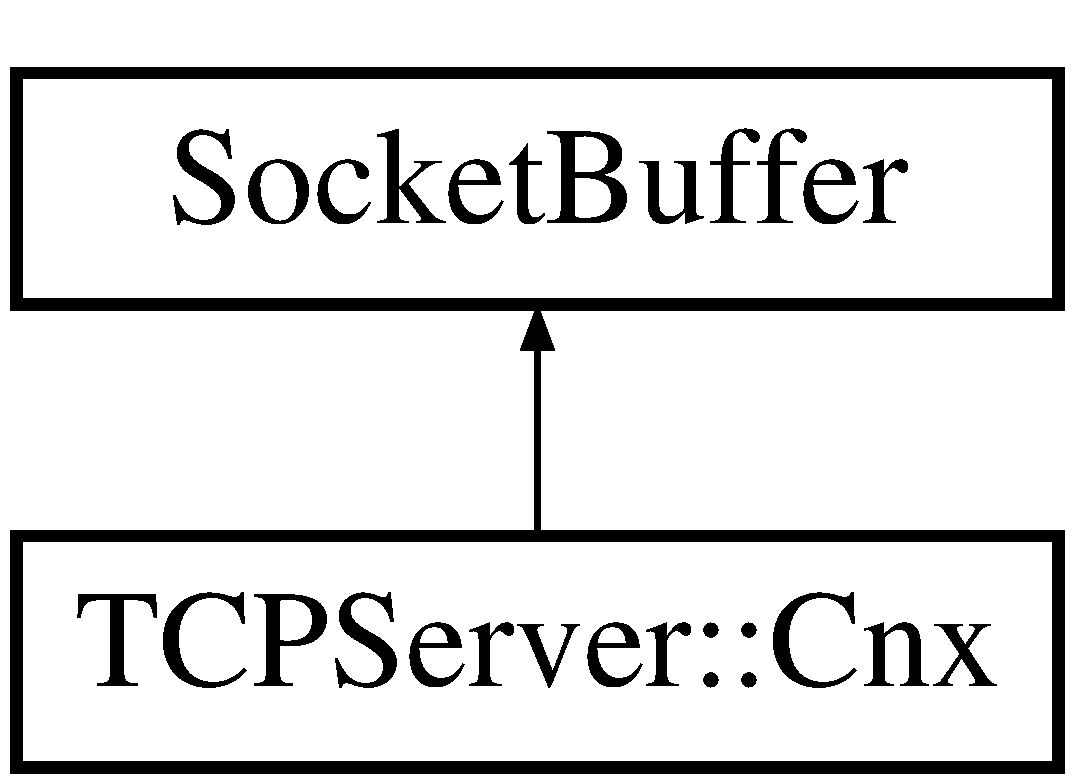
\includegraphics[height=2.000000cm]{class_socket_buffer}
\end{center}
\end{figure}
\subsection*{Public Member Functions}
\begin{DoxyCompactItemize}
\item 
\hyperlink{class_socket_buffer_aa9ed1cc8e166f53606b31246838b3d87}{Socket\+Buffer} (\hyperlink{class_socket}{Socket} $\ast$socket, size\+\_\+t input\+Buffer\+Size=8192, size\+\_\+t ouput\+Buffer\+Size=8192)\hypertarget{class_socket_buffer_aa9ed1cc8e166f53606b31246838b3d87}{}\label{class_socket_buffer_aa9ed1cc8e166f53606b31246838b3d87}

\begin{DoxyCompactList}\small\item\em constructor. The argument must be a valid connected T\+C\+P/\+IP \hyperlink{class_socket}{Socket} (i.\+e. of S\+O\+C\+K\+\_\+\+S\+T\+R\+E\+AM type) that must N\+OT be destructed while this \hyperlink{class_socket_buffer}{Socket\+Buffer} is used. \end{DoxyCompactList}\item 
{\bfseries Socket\+Buffer} (\hyperlink{class_socket}{Socket} \&socket, size\+\_\+t input\+Buffer\+Size=8192, size\+\_\+t ouput\+Buffer\+Size=8192)\hypertarget{class_socket_buffer_a40ad003b90446f69fb0fa4cc18c0d28b}{}\label{class_socket_buffer_a40ad003b90446f69fb0fa4cc18c0d28b}

\item 
\hyperlink{class_socket}{Socket} $\ast$ {\bfseries socket} ()\hypertarget{class_socket_buffer_aa9c14ec14e092fc58c4363d2bbc20ffd}{}\label{class_socket_buffer_aa9c14ec14e092fc58c4363d2bbc20ffd}

\item 
virtual void \hyperlink{class_socket_buffer_ac03353a864ab3a04aa25364a333c0a09}{set\+Separators} (int input\+Separator, int output\+Separator)
\begin{DoxyCompactList}\small\item\em changes the Line Separators. the argument is a character or a negative value (see below)\+: \end{DoxyCompactList}\item 
virtual void \hyperlink{class_socket_buffer_a81a280c639a913b5dbfb12611f339232}{get\+Separators} (int \&input\+Separator, int \&output\+Separator) const 
\begin{DoxyCompactList}\small\item\em returns the Line Separators. \end{DoxyCompactList}\item 
virtual ssize\+\_\+t \hyperlink{class_socket_buffer_a279a372ca946b58455dba0e9c12e213d}{read\+Line} (std\+::string \&str)
\begin{DoxyCompactList}\small\item\em Reads a line of text from a connected socket. The text is stored in the string given as an argument. The other side must send a line of text ended by a Line Separator (. \end{DoxyCompactList}\item 
virtual ssize\+\_\+t \hyperlink{class_socket_buffer_af589c1459da6bca39badf56798c6f859}{write\+Line} (const std\+::string \&str)
\begin{DoxyCompactList}\small\item\em Sends a line of text to a connected socket. Sends the string given as an argument. A Line Separator is automatically added (. \end{DoxyCompactList}\item 
virtual ssize\+\_\+t {\bfseries read} (char $\ast$buffer, size\+\_\+t len)\hypertarget{class_socket_buffer_ab77a4365cfb9625dc996005ffa22bc0c}{}\label{class_socket_buffer_ab77a4365cfb9625dc996005ffa22bc0c}

\item 
virtual ssize\+\_\+t {\bfseries write} (const char $\ast$str, size\+\_\+t len)\hypertarget{class_socket_buffer_a2ceb624ffd27a27ef500574646c9a8fa}{}\label{class_socket_buffer_a2ceb624ffd27a27ef500574646c9a8fa}

\end{DoxyCompactItemize}
\subsection*{Protected Member Functions}
\begin{DoxyCompactItemize}
\item 
virtual bool {\bfseries retrieve\+Line} (std\+::string \&str, ssize\+\_\+t received)\hypertarget{class_socket_buffer_ab2f6ba1d14564967e1714ddd478275d8}{}\label{class_socket_buffer_ab2f6ba1d14564967e1714ddd478275d8}

\end{DoxyCompactItemize}
\subsection*{Protected Attributes}
\begin{DoxyCompactItemize}
\item 
size\+\_\+t {\bfseries \+\_\+in\+Size}\hypertarget{class_socket_buffer_a19f587689e24a3900a4157be5fa27205}{}\label{class_socket_buffer_a19f587689e24a3900a4157be5fa27205}

\item 
size\+\_\+t {\bfseries \+\_\+out\+Size}\hypertarget{class_socket_buffer_a1ce4a460af7a7fb2f3609bcb9f15ece7}{}\label{class_socket_buffer_a1ce4a460af7a7fb2f3609bcb9f15ece7}

\item 
int {\bfseries \+\_\+in\+Sep}\hypertarget{class_socket_buffer_a8958b13b28d476081c10aac8e25a87d2}{}\label{class_socket_buffer_a8958b13b28d476081c10aac8e25a87d2}

\item 
int {\bfseries \+\_\+out\+Sep}\hypertarget{class_socket_buffer_add088335eb098a067980157b310b22cb}{}\label{class_socket_buffer_add088335eb098a067980157b310b22cb}

\item 
\hyperlink{class_socket}{Socket} $\ast$ {\bfseries \+\_\+sock}\hypertarget{class_socket_buffer_a8575c3a91db81fac18e5634c427faafb}{}\label{class_socket_buffer_a8575c3a91db81fac18e5634c427faafb}

\item 
struct \hyperlink{struct_input_buffer}{Input\+Buffer} $\ast$ {\bfseries \+\_\+in}\hypertarget{class_socket_buffer_a8cf67350de772512eff4af7d7f378bed}{}\label{class_socket_buffer_a8cf67350de772512eff4af7d7f378bed}

\end{DoxyCompactItemize}


\subsection{Detailed Description}
Class for exchanging text strings between T\+C\+P/\+IP sockets. T\+C\+P/\+IP connected sockets do not preserve record boundaries. Messages can be split or merged so that one call to \hyperlink{class_socket_a9275eacdb64056a53cf4b9cf54cd2f1a}{Socket\+::send()} on the sending side does not necessarily correspond to one call to \hyperlink{class_socket_aa5e98b6f2c4e26fcf90d71c8386fc09d}{Socket\+::receive()} on the receiving side. 

The methods of this class solve this problem\+:
\begin{DoxyItemize}
\item by calling \hyperlink{class_socket_a9275eacdb64056a53cf4b9cf54cd2f1a}{Socket\+::send()} or \hyperlink{class_socket_aa5e98b6f2c4e26fcf90d71c8386fc09d}{Socket\+::receive()} as many times as needed
\item by using a Line Separator to separate text lines (\begin{DoxySeeAlso}{See also}
set\+Separator()) 
\end{DoxySeeAlso}

\end{DoxyItemize}

\subsection{Member Function Documentation}
\index{Socket\+Buffer@{Socket\+Buffer}!get\+Separators@{get\+Separators}}
\index{get\+Separators@{get\+Separators}!Socket\+Buffer@{Socket\+Buffer}}
\subsubsection[{\texorpdfstring{get\+Separators(int \&input\+Separator, int \&output\+Separator) const }{getSeparators(int &inputSeparator, int &outputSeparator) const }}]{\setlength{\rightskip}{0pt plus 5cm}void Socket\+Buffer\+::get\+Separators (
\begin{DoxyParamCaption}
\item[{int \&}]{input\+Separator, }
\item[{int \&}]{output\+Separator}
\end{DoxyParamCaption}
) const\hspace{0.3cm}{\ttfamily [virtual]}}\hypertarget{class_socket_buffer_a81a280c639a913b5dbfb12611f339232}{}\label{class_socket_buffer_a81a280c639a913b5dbfb12611f339232}


returns the Line Separators. 

\begin{DoxySeeAlso}{See also}
\hyperlink{class_socket_buffer_ac03353a864ab3a04aa25364a333c0a09}{set\+Separators()}. 
\end{DoxySeeAlso}
\index{Socket\+Buffer@{Socket\+Buffer}!read\+Line@{read\+Line}}
\index{read\+Line@{read\+Line}!Socket\+Buffer@{Socket\+Buffer}}
\subsubsection[{\texorpdfstring{read\+Line(std\+::string \&str)}{readLine(std::string &str)}}]{\setlength{\rightskip}{0pt plus 5cm}ssize\+\_\+t Socket\+Buffer\+::read\+Line (
\begin{DoxyParamCaption}
\item[{std\+::string \&}]{str}
\end{DoxyParamCaption}
)\hspace{0.3cm}{\ttfamily [virtual]}}\hypertarget{class_socket_buffer_a279a372ca946b58455dba0e9c12e213d}{}\label{class_socket_buffer_a279a372ca946b58455dba0e9c12e213d}


Reads a line of text from a connected socket. The text is stored in the string given as an argument. The other side must send a line of text ended by a Line Separator (. 

\begin{DoxySeeAlso}{See also}
set\+Separator()) which is automatically done by \hyperlink{class_socket_buffer_af589c1459da6bca39badf56798c6f859}{write\+Line()}. The separator is not stored in the argument. 
\end{DoxySeeAlso}
\begin{DoxyReturn}{Returns}
the number of bytes that was received (including the separator) except if\+:
\begin{DoxyItemize}
\item shutdown\+Output() was called on the other side (0 is returned)
\item an error occured (Socket\+::\+Failed is returned)
\item the socket is invalid (Socket\+::\+Invalid\+Socket is returned) 
\end{DoxyItemize}
\end{DoxyReturn}
\begin{DoxyNote}{Note}
this method may block. 
\end{DoxyNote}
\index{Socket\+Buffer@{Socket\+Buffer}!set\+Separators@{set\+Separators}}
\index{set\+Separators@{set\+Separators}!Socket\+Buffer@{Socket\+Buffer}}
\subsubsection[{\texorpdfstring{set\+Separators(int input\+Separator, int output\+Separator)}{setSeparators(int inputSeparator, int outputSeparator)}}]{\setlength{\rightskip}{0pt plus 5cm}void Socket\+Buffer\+::set\+Separators (
\begin{DoxyParamCaption}
\item[{int}]{input\+Separator, }
\item[{int}]{output\+Separator}
\end{DoxyParamCaption}
)\hspace{0.3cm}{\ttfamily [virtual]}}\hypertarget{class_socket_buffer_ac03353a864ab3a04aa25364a333c0a09}{}\label{class_socket_buffer_ac03353a864ab3a04aa25364a333c0a09}


changes the Line Separators. the argument is a character or a negative value (see below)\+: 


\begin{DoxyItemize}
\item if {\itshape input\+Separator} is $<$ 0 (the default) a line is considered to be terminated by any one of \textquotesingle{}~\newline
\textquotesingle{} or \textquotesingle{}\textquotesingle{} or \textquotesingle{}~\newline
\textquotesingle{} followed by \textquotesingle{}\textquotesingle{}
\item if {\itshape output\+Separator} is $<$ 0 a line is terminated by \textquotesingle{}~\newline
\textquotesingle{} followed by \textquotesingle{}\textquotesingle{}. The default value is \textquotesingle{}~\newline
\textquotesingle{}. 
\end{DoxyItemize}\index{Socket\+Buffer@{Socket\+Buffer}!write\+Line@{write\+Line}}
\index{write\+Line@{write\+Line}!Socket\+Buffer@{Socket\+Buffer}}
\subsubsection[{\texorpdfstring{write\+Line(const std\+::string \&str)}{writeLine(const std::string &str)}}]{\setlength{\rightskip}{0pt plus 5cm}ssize\+\_\+t Socket\+Buffer\+::write\+Line (
\begin{DoxyParamCaption}
\item[{const std\+::string \&}]{str}
\end{DoxyParamCaption}
)\hspace{0.3cm}{\ttfamily [virtual]}}\hypertarget{class_socket_buffer_af589c1459da6bca39badf56798c6f859}{}\label{class_socket_buffer_af589c1459da6bca39badf56798c6f859}


Sends a line of text to a connected socket. Sends the string given as an argument. A Line Separator is automatically added (. 

\begin{DoxySeeAlso}{See also}
set\+Separator()). 
\end{DoxySeeAlso}
\begin{DoxyReturn}{Returns}
the number of bytes that was sent (including the separator) except if\+:
\begin{DoxyItemize}
\item shutdown\+Input() was called on the other side (0 is returned)
\item an error occured (Socket\+::\+Failed is returned)
\item the socket is invalid (Socket\+::\+Invalid\+Socket is returned) 
\end{DoxyItemize}
\end{DoxyReturn}
\begin{DoxyNote}{Note}
this method may block. 
\end{DoxyNote}


The documentation for this class was generated from the following files\+:\begin{DoxyCompactItemize}
\item 
C\+:/\+Users/\+Will/\+Desktop/\+Ung\+William/cpp/Socket.\+h\item 
C\+:/\+Users/\+Will/\+Desktop/\+Ung\+William/cpp/Socket.\+cpp\end{DoxyCompactItemize}

\hypertarget{class_t_c_p_server}{}\section{T\+C\+P\+Server Class Reference}
\label{class_t_c_p_server}\index{T\+C\+P\+Server@{T\+C\+P\+Server}}


T\+C\+P/\+IP I\+Pv4 server. The server supports T\+C\+P/\+IP A\+F\+\_\+\+I\+N\+ET connections (following the I\+Pv4 Internet protocol) with multiple clients. One thread is used per client.  




{\ttfamily \#include $<$T\+C\+P\+Server.\+h$>$}

\subsection*{Classes}
\begin{DoxyCompactItemize}
\item 
class \hyperlink{class_t_c_p_server_1_1_callback}{Callback}
\item 
class \hyperlink{class_t_c_p_server_1_1_callback_impl}{Callback\+Impl}
\item 
class \hyperlink{class_t_c_p_server_1_1_cnx}{Cnx}
\begin{DoxyCompactList}\small\item\em represents a connection with a given client. \end{DoxyCompactList}\item 
class \hyperlink{class_t_c_p_server_1_1_lock}{Lock}
\begin{DoxyCompactList}\small\item\em locks the server in read mode or in write mode. In order to avoid concurrency problems between threads, the callback method that processes requests should instantiate a \hyperlink{class_t_c_p_server_1_1_lock}{Lock} object in the stack. The \hyperlink{class_t_c_p_server_1_1_lock}{Lock} must be instantiated in write mode if the request changes data, or in read mode otherwise. A write lock blocks all other locks (hence, all other threads) until the callback method that issued the write lock returns. \end{DoxyCompactList}\end{DoxyCompactItemize}
\subsection*{Public Member Functions}
\begin{DoxyCompactItemize}
\item 
\hyperlink{class_t_c_p_server_a3a5e3cfe42c676ed71f2bc58dcc92bda}{T\+C\+P\+Server} ()\hypertarget{class_t_c_p_server_a3a5e3cfe42c676ed71f2bc58dcc92bda}{}\label{class_t_c_p_server_a3a5e3cfe42c676ed71f2bc58dcc92bda}

\begin{DoxyCompactList}\small\item\em constructor\+: initializes the \hyperlink{class_t_c_p_server}{T\+C\+P\+Server}. \end{DoxyCompactList}\item 
virtual \hyperlink{class_t_c_p_server_abc497ac52355e53986a6a1bd1acb9581}{$\sim$\+T\+C\+P\+Server} ()\hypertarget{class_t_c_p_server_abc497ac52355e53986a6a1bd1acb9581}{}\label{class_t_c_p_server_abc497ac52355e53986a6a1bd1acb9581}

\begin{DoxyCompactList}\small\item\em destructor\+: cleans up the \hyperlink{class_t_c_p_server}{T\+C\+P\+Server}. \end{DoxyCompactList}\item 
virtual int \hyperlink{class_t_c_p_server_a1409041961e91f1dbc4933483b4c3b23}{run} (int port)
\begin{DoxyCompactList}\small\item\em starts the main loop of the server on this port. This function binds an internal \hyperlink{class_server_socket}{Server\+Socket} then starts an infinite main loop that receives requests from clients. The function creates one thread per client. \end{DoxyCompactList}\item 
{\footnotesize template$<$class T $>$ }\\void \hyperlink{class_t_c_p_server_ac62c8c7a1d1137b74e2a1fa6d8a4a876}{set\+Callback} (T $\ast$obj, bool(T\+::$\ast$func)(\hyperlink{class_t_c_p_server_1_1_cnx}{Cnx} \&, const std\+::string \&request, std\+::string \&response))
\begin{DoxyCompactList}\small\item\em changes the callback method that processes requests. The first argument must be an object, the second argument a method of this object. This method will be called each time the \hyperlink{class_t_c_p_server}{T\+C\+P\+Server} receives a \textquotesingle{}request\textquotesingle{} from a client in order to perform a computation and return a \textquotesingle{}response\textquotesingle{} to this client. \end{DoxyCompactList}\end{DoxyCompactItemize}
\subsection*{Protected Member Functions}
\begin{DoxyCompactItemize}
\item 
virtual void \hyperlink{class_t_c_p_server_af99977f3ec05210e91d02aa9c693254b}{read\+Messages} (\hyperlink{class_t_c_p_server_1_1_cnx}{T\+C\+P\+Server\+::\+Cnx} $\ast$)\hypertarget{class_t_c_p_server_af99977f3ec05210e91d02aa9c693254b}{}\label{class_t_c_p_server_af99977f3ec05210e91d02aa9c693254b}

\begin{DoxyCompactList}\small\item\em reads messages from a given client on the corresponding thread. \end{DoxyCompactList}\item 
virtual void \hyperlink{class_t_c_p_server_a2f053dfc720aab308f97ccc8a789adc4}{print\+Msg} (const std\+::string \&msg, const \hyperlink{class_t_c_p_server_1_1_cnx}{T\+C\+P\+Server\+::\+Cnx} $\ast$=0)\hypertarget{class_t_c_p_server_a2f053dfc720aab308f97ccc8a789adc4}{}\label{class_t_c_p_server_a2f053dfc720aab308f97ccc8a789adc4}

\begin{DoxyCompactList}\small\item\em prints warning and error messages on the terminal. \end{DoxyCompactList}\end{DoxyCompactItemize}
\subsection*{Protected Attributes}
\begin{DoxyCompactItemize}
\item 
\hyperlink{class_server_socket}{Server\+Socket} {\bfseries \+\_\+servsock}\hypertarget{class_t_c_p_server_a9c2891cf40b19735bceb22605a5e867e}{}\label{class_t_c_p_server_a9c2891cf40b19735bceb22605a5e867e}

\item 
std\+::shared\+\_\+ptr$<$ \hyperlink{class_t_c_p_server_1_1_callback}{Callback} $>$ {\bfseries \+\_\+callback}\hypertarget{class_t_c_p_server_a1f7a87b1f42950325d005c8a0ca9427e}{}\label{class_t_c_p_server_a1f7a87b1f42950325d005c8a0ca9427e}

\item 
pthread\+\_\+rwlock\+\_\+t {\bfseries \+\_\+threadlock}\hypertarget{class_t_c_p_server_a130152438b313a1c4470c842a063257d}{}\label{class_t_c_p_server_a130152438b313a1c4470c842a063257d}

\end{DoxyCompactItemize}


\subsection{Detailed Description}
T\+C\+P/\+IP I\+Pv4 server. The server supports T\+C\+P/\+IP A\+F\+\_\+\+I\+N\+ET connections (following the I\+Pv4 Internet protocol) with multiple clients. One thread is used per client. 

The \hyperlink{class_t_c_p_server_a1409041961e91f1dbc4933483b4c3b23}{run()} method binds an internal \hyperlink{class_server_socket}{Server\+Socket} then starts an infinite main loop that receives requests from clients. Requests can be received concurrently thanks to threads.

A callback method is called each time the sever receives a request from a client (\begin{DoxySeeAlso}{See also}
\hyperlink{class_t_c_p_server_ac62c8c7a1d1137b74e2a1fa6d8a4a876}{set\+Callback()} to set this method). This method can issue read and write locks to avoid concurrency issues (

\hyperlink{class_t_c_p_server_1_1_lock}{Lock}). 
\end{DoxySeeAlso}


\subsection{Member Function Documentation}
\index{T\+C\+P\+Server@{T\+C\+P\+Server}!run@{run}}
\index{run@{run}!T\+C\+P\+Server@{T\+C\+P\+Server}}
\subsubsection[{\texorpdfstring{run(int port)}{run(int port)}}]{\setlength{\rightskip}{0pt plus 5cm}int T\+C\+P\+Server\+::run (
\begin{DoxyParamCaption}
\item[{int}]{port}
\end{DoxyParamCaption}
)\hspace{0.3cm}{\ttfamily [virtual]}}\hypertarget{class_t_c_p_server_a1409041961e91f1dbc4933483b4c3b23}{}\label{class_t_c_p_server_a1409041961e91f1dbc4933483b4c3b23}


starts the main loop of the server on this port. This function binds an internal \hyperlink{class_server_socket}{Server\+Socket} then starts an infinite main loop that receives requests from clients. The function creates one thread per client. 

\begin{DoxyReturn}{Returns}
0 on normal termination or a negative value if the \hyperlink{class_server_socket}{Server\+Socket} could not be bound (value is then one of \hyperlink{class_socket_a9f68308228badcdd299cd83e62e36976}{Socket\+::\+Errors}). 
\end{DoxyReturn}
\index{T\+C\+P\+Server@{T\+C\+P\+Server}!set\+Callback@{set\+Callback}}
\index{set\+Callback@{set\+Callback}!T\+C\+P\+Server@{T\+C\+P\+Server}}
\subsubsection[{\texorpdfstring{set\+Callback(\+T $\ast$obj, bool(\+T\+::$\ast$func)(\+Cnx \&, const std\+::string \&request, std\+::string \&response))}{setCallback(T *obj, bool(T::*func)(Cnx &, const std::string &request, std::string &response))}}]{\setlength{\rightskip}{0pt plus 5cm}template$<$class T $>$ void T\+C\+P\+Server\+::set\+Callback (
\begin{DoxyParamCaption}
\item[{T $\ast$}]{obj, }
\item[{bool(T\+::$\ast$)({\bf Cnx} \&, const std\+::string \&request, std\+::string \&response)}]{func}
\end{DoxyParamCaption}
)\hspace{0.3cm}{\ttfamily [inline]}}\hypertarget{class_t_c_p_server_ac62c8c7a1d1137b74e2a1fa6d8a4a876}{}\label{class_t_c_p_server_ac62c8c7a1d1137b74e2a1fa6d8a4a876}


changes the callback method that processes requests. The first argument must be an object, the second argument a method of this object. This method will be called each time the \hyperlink{class_t_c_p_server}{T\+C\+P\+Server} receives a \textquotesingle{}request\textquotesingle{} from a client in order to perform a computation and return a \textquotesingle{}response\textquotesingle{} to this client. 

Arguments and return value of the method\+:
\begin{DoxyItemize}
\item the \textquotesingle{}request\textquotesingle{} and the \textquotesingle{}response\textquotesingle{} are provided through the corresponding parameters of the method.
\item the connection with the client will be closed if the method returns false 
\end{DoxyItemize}

The documentation for this class was generated from the following files\+:\begin{DoxyCompactItemize}
\item 
C\+:/\+Users/\+Will/\+Desktop/\+Ung\+William/cpp/T\+C\+P\+Server.\+h\item 
C\+:/\+Users/\+Will/\+Desktop/\+Ung\+William/cpp/T\+C\+P\+Server.\+cpp\end{DoxyCompactItemize}

\hypertarget{class_video}{}\section{Video Class Reference}
\label{class_video}\index{Video@{Video}}
Inheritance diagram for Video\+:\begin{figure}[H]
\begin{center}
\leavevmode
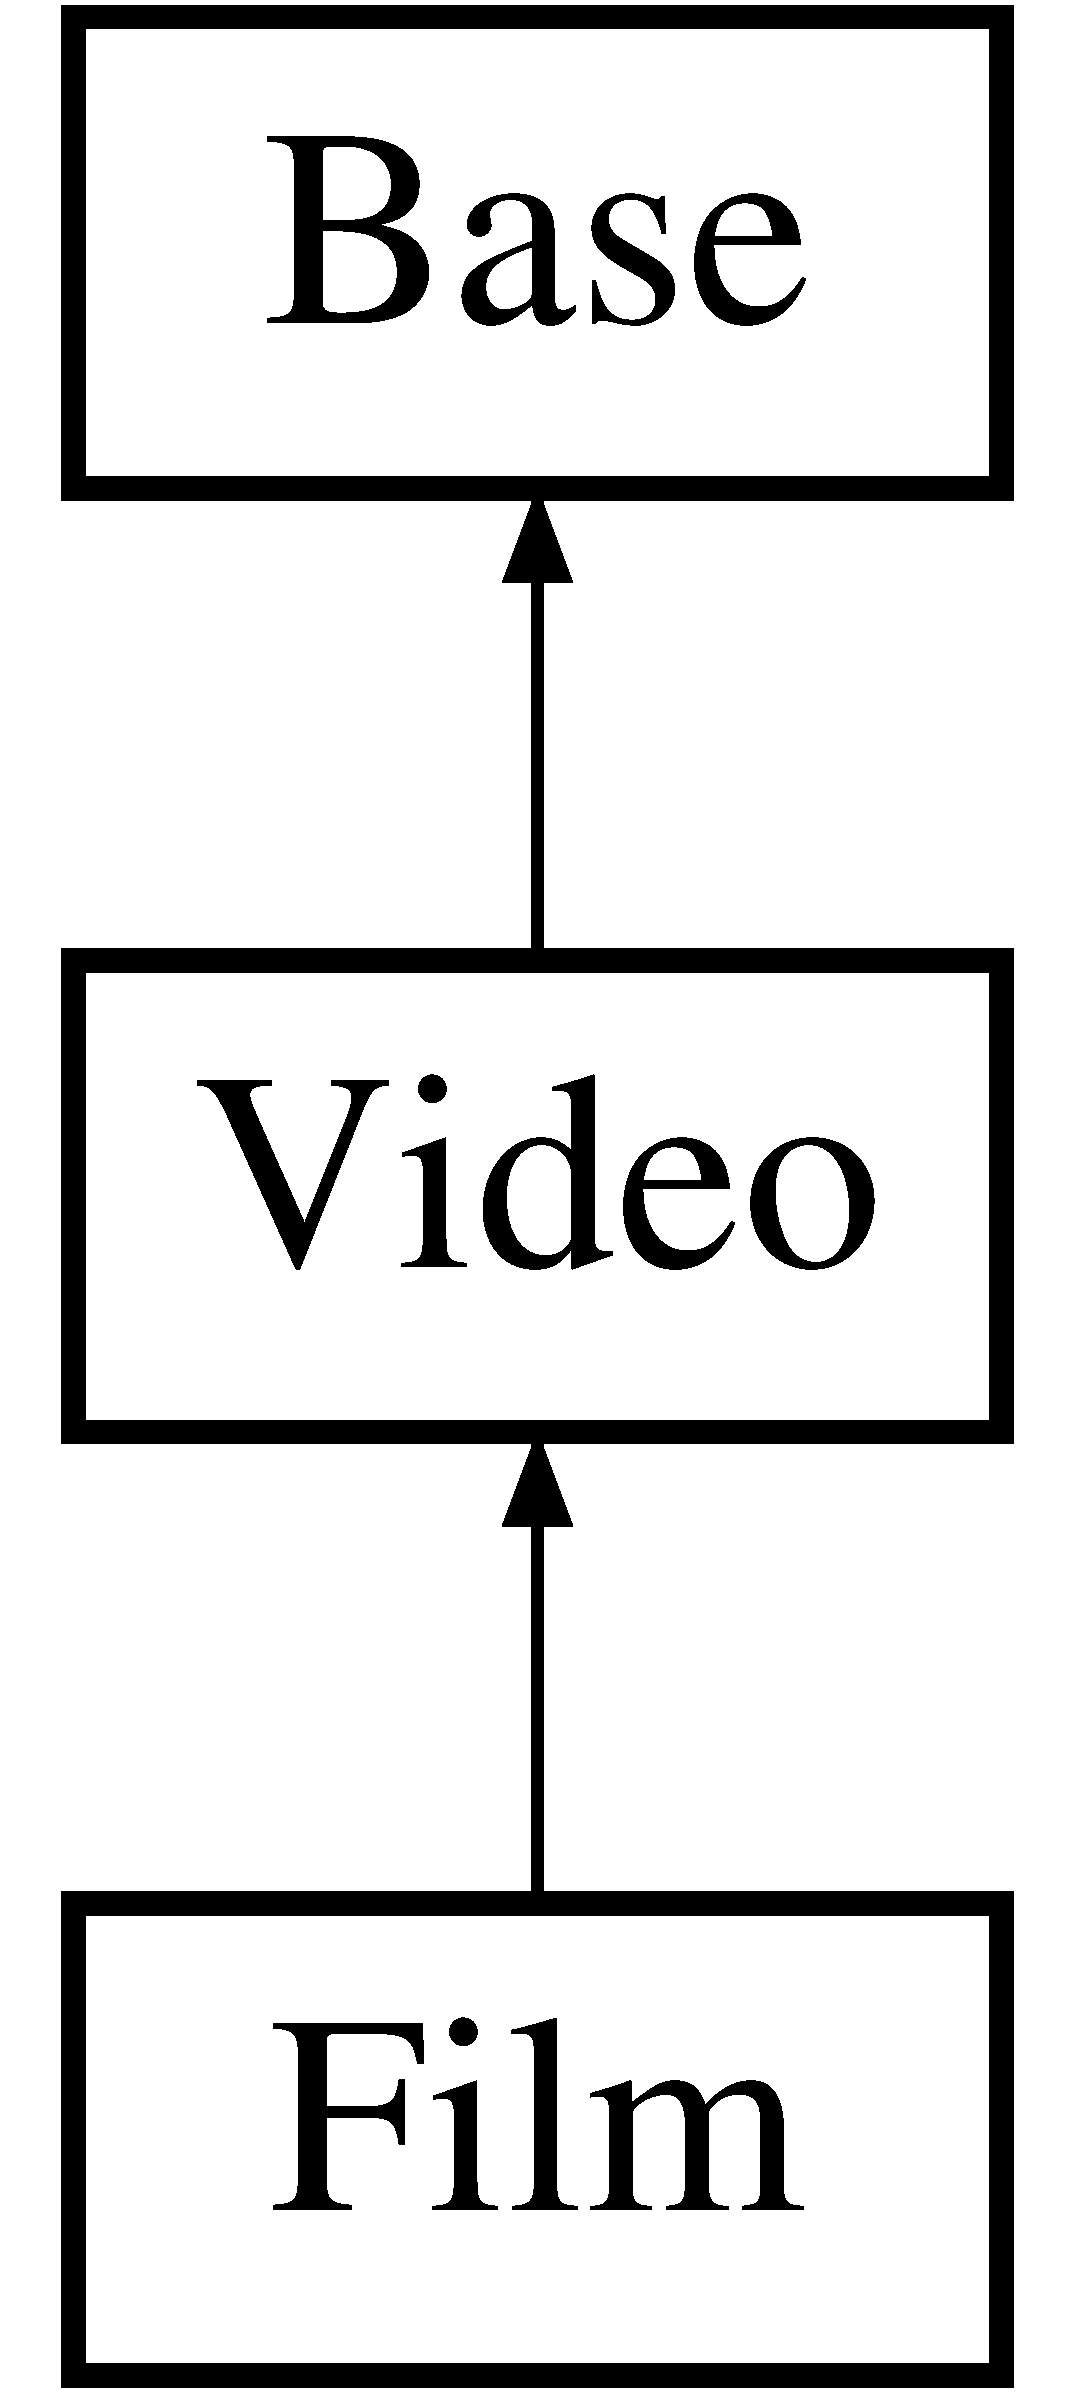
\includegraphics[height=3.000000cm]{class_video}
\end{center}
\end{figure}
\subsection*{Public Member Functions}
\begin{DoxyCompactItemize}
\item 
{\bfseries Video} (string obj, string pat, int \+\_\+duree=0)\hypertarget{class_video_ae95cc353bcad4987de49bfe8dfb6c4fb}{}\label{class_video_ae95cc353bcad4987de49bfe8dfb6c4fb}

\item 
unsigned int {\bfseries get\+Duree} () const \hypertarget{class_video_ac9ed820535234a8c6520f68a60e72a61}{}\label{class_video_ac9ed820535234a8c6520f68a60e72a61}

\item 
void {\bfseries set\+Duree} (unsigned int dur)\hypertarget{class_video_a42f10c74a3bf8839d19ab9b1e8954f0a}{}\label{class_video_a42f10c74a3bf8839d19ab9b1e8954f0a}

\item 
virtual void {\bfseries print} (ostream \&os) override\hypertarget{class_video_ae527f70f5ddf9195d45b33710af6cdb7}{}\label{class_video_ae527f70f5ddf9195d45b33710af6cdb7}

\item 
virtual void {\bfseries play} () override\hypertarget{class_video_a70e78dc07cccb122b0a387488f9f7d8e}{}\label{class_video_a70e78dc07cccb122b0a387488f9f7d8e}

\end{DoxyCompactItemize}
\subsection*{Protected Attributes}
\begin{DoxyCompactItemize}
\item 
unsigned int {\bfseries duree}\hypertarget{class_video_a16ecfab926b5c3532b02471653212ed8}{}\label{class_video_a16ecfab926b5c3532b02471653212ed8}

\end{DoxyCompactItemize}


The documentation for this class was generated from the following file\+:\begin{DoxyCompactItemize}
\item 
C\+:/\+Users/\+Will/\+Desktop/\+Ung\+William/cpp/Video.\+h\end{DoxyCompactItemize}

\hypertarget{class_x_maps}{}\section{X\+Maps Class Reference}
\label{class_x_maps}\index{X\+Maps@{X\+Maps}}
\subsection*{Public Member Functions}
\begin{DoxyCompactItemize}
\item 
sp\+Photo {\bfseries add\+Photo} (string key)\hypertarget{class_x_maps_a1f18863c96ddb7cd210d59c2b59846c6}{}\label{class_x_maps_a1f18863c96ddb7cd210d59c2b59846c6}

\item 
sp\+Video {\bfseries add\+Video} (string key)\hypertarget{class_x_maps_ac91c419ae96c6335606a4e840e1eeadc}{}\label{class_x_maps_ac91c419ae96c6335606a4e840e1eeadc}

\item 
sp\+Film {\bfseries add\+Film} (string key)\hypertarget{class_x_maps_a7364d8cfd45a1575d0d2cbf8bd53edef}{}\label{class_x_maps_a7364d8cfd45a1575d0d2cbf8bd53edef}

\item 
sp\+Groupe {\bfseries add\+Groupe\+Map} (string key)\hypertarget{class_x_maps_a648a31f57c14f71144822955c608ae8b}{}\label{class_x_maps_a648a31f57c14f71144822955c608ae8b}

\item 
void {\bfseries remove\+Base} (string key)\hypertarget{class_x_maps_a330f1b77f89e5707d210bc6f6ee3a12d}{}\label{class_x_maps_a330f1b77f89e5707d210bc6f6ee3a12d}

\item 
void {\bfseries remove\+Groupe} (string key)\hypertarget{class_x_maps_aca8175e95bf520bfe67cb6d9632ae481}{}\label{class_x_maps_aca8175e95bf520bfe67cb6d9632ae481}

\item 
void {\bfseries search\+Base} (string key, ostream \&os)\hypertarget{class_x_maps_adb1054a64b0bf297d9ddd5e5ce59a33e}{}\label{class_x_maps_adb1054a64b0bf297d9ddd5e5ce59a33e}

\item 
void {\bfseries search\+Groupe} (string key, ostream \&os)\hypertarget{class_x_maps_a5133e8a7a2ff162b7b984510be80efca}{}\label{class_x_maps_a5133e8a7a2ff162b7b984510be80efca}

\item 
void {\bfseries play\+Base} (string key)\hypertarget{class_x_maps_aa95ef3f9ad5257840d85e00c1d6d8778}{}\label{class_x_maps_aa95ef3f9ad5257840d85e00c1d6d8778}

\item 
string {\bfseries find} (string key)\hypertarget{class_x_maps_af9e00ed252d47df69f70c6d99a964195}{}\label{class_x_maps_af9e00ed252d47df69f70c6d99a964195}

\item 
bool {\bfseries process\+Request} (\hyperlink{class_t_c_p_server_1_1_cnx}{T\+C\+P\+Server\+::\+Cnx} \&cnx, const string \&request, string \&response)\hypertarget{class_x_maps_a95715b70da3dcef748fa46ead88613ca}{}\label{class_x_maps_a95715b70da3dcef748fa46ead88613ca}

\end{DoxyCompactItemize}
\subsection*{Protected Attributes}
\begin{DoxyCompactItemize}
\item 
map$<$ string, sp\+Base $>$ {\bfseries base\+Map}\hypertarget{class_x_maps_a294c98cacd43c3015de8fc51de4e493f}{}\label{class_x_maps_a294c98cacd43c3015de8fc51de4e493f}

\item 
map$<$ string, sp\+Groupe $>$ {\bfseries groupe\+Map}\hypertarget{class_x_maps_a341528368e04f64f7cb62eb21a120f3a}{}\label{class_x_maps_a341528368e04f64f7cb62eb21a120f3a}

\end{DoxyCompactItemize}


The documentation for this class was generated from the following files\+:\begin{DoxyCompactItemize}
\item 
C\+:/\+Users/\+Will/\+Desktop/\+Ung\+William/cpp/X\+Maps.\+h\item 
C\+:/\+Users/\+Will/\+Desktop/\+Ung\+William/cpp/X\+Maps.\+cpp\end{DoxyCompactItemize}

%--- End generated contents ---

% Index
\backmatter
\newpage
\phantomsection
\clearemptydoublepage
\addcontentsline{toc}{chapter}{Index}
\printindex

\end{document}
